\documentclass[11pt, oneside]{article}      % use "amsart" instead of "article" for AMSLaTeX format
% \usepackage{geometry}                       % See geometry.pdf to learn the layout options. There are lots.
% \geometry{letterpaper}                          % ... or a4paper or a5paper or ... 
%\geometry{landscape}                       % Activate for rotated page geometry
%\usepackage[parfill]{parskip}          	% Activate to begin paragraphs with an empty line rather than an indent
\usepackage{graphicx}
\usepackage{amsmath,amsthm,amssymb}
\usepackage{mathtools}
\usepackage{xcolor}
\usepackage[font=small,labelfont=bf,skip=0pt,justification=justified]{caption}
\usepackage{stackengine}
% \usepackage{natbib}
\usepackage{stmaryrd}
\usepackage[most]{tcolorbox}
\usepackage{tikzit}
\input{zx.tikzdefs}
\input{zx.tikzstyles}

\usepackage{hyperref} % must be last package used

% \bibliographystyle{abbrvnat}
% \setcitestyle{square, authoryear}
% \setlength{\parindent}{0in}
% \setcitestyle{square}
\theoremstyle{definition}
\newtheorem{theorem}{Theorem}[section]
\newtheorem{corollary}[theorem]{Corollary}
\newtheorem{lemma}[theorem]{Lemma}
\newtheorem*{lemma*}{Lemma}
\newtheorem*{proposition*}{Proposition}
\newtheorem{proposition}[theorem]{Proposition}
\newtheorem{conjecture}[theorem]{Conjecture}
\newtheorem{definition}[theorem]{Definition}
\newtheorem{example}[theorem]{Example}
\newtheorem{remark}[theorem]{Remark}
\newtheorem{warning}[theorem]{Warning}

\newcommand{\defeq}{\vcentcolon=}
\newcommand{\eqdef}{=\vcentcolon}
\newcommand{\xeq}[1]{\mathrel{\stackon[5pt]{$=$}{$\scriptstyle{#1}$}}}
\newcommand{\xeqq}[2]{\mathrel{\stackon[5pt]{$=$}{\stackon[5pt]{$\scriptstyle{#1}$}{$\scriptstyle{#2}$}}}}
\newcommand{\abs}[1]{\ensuremath{\lvert #1 \rvert}}

\newcommand{\qutritZphase}[2]{\,\tikz{\node[style=qutrit Z phase] (x) {$#1$ \nodepart{lower} $#2$};}\,}
\newcommand{\qutritXphase}[2]{\,\tikz{\node[style=qutrit X phase] (x) {$#1$ \nodepart{lower} $#2$};}\,}

\newcommand{\qutritZspider}[2]{\,\begin{tikzpicture}
	\begin{pgfonlayer}{nodelayer}
		\node [style=none] (1) at (0, 0.75) {...};
		\node [style=none] (5) at (-0.75, 1) {};
		\node [style=none] (7) at (0.75, 1) {};
		\node [style=none] (8) at (0, -0.75) {...};
		\node [style=none] (9) at (-0.75, -1) {};
		\node [style=qutrit Z phase] (10) at (0, 0) {$#1$ \nodepart{lower} $#2$};
		\node [style=none] (11) at (0.75, -1) {};
	\end{pgfonlayer}
	\begin{pgfonlayer}{edgelayer}
		\draw [bend left=15] (10) to (11.center);
		\draw [bend right=15] (10) to (9.center);
		\draw [bend right=15] (10) to (7.center);
		\draw [bend left=15] (10) to (5.center);
	\end{pgfonlayer}
\end{tikzpicture}}
\newcommand{\qutritState}[3]{\, \begin{tikzpicture}
	\begin{pgfonlayer}{nodelayer}
		\node [style=none] (1) at (0, 0.75) {};
		\node [style=qutrit #1 phase] (2) at (0, -0.5) {$#2$ \nodepart{lower} $#3$};
	\end{pgfonlayer}
	\begin{pgfonlayer}{edgelayer}
		\draw (1.center) to (2);
	\end{pgfonlayer}
\end{tikzpicture}}
\newcommand{\qutritZstate}[2]{\qutritState{Z}{#1}{#2}}
\newcommand{\qutritXstate}[2]{\qutritState{X}{#1}{#2}}

\newcommand{\qubitPhaseGate}[2]{\,\begin{tikzpicture}
	\begin{pgfonlayer}{nodelayer}
		\node [style=#1 phase dot] (0) at (0, 0) {$#2$};
		\node [style=none] (1) at (0, 1) {};
		\node [style=none] (2) at (0, -1) {};
	\end{pgfonlayer}
	\begin{pgfonlayer}{edgelayer}
		\draw (1.center) to (2.center);
	\end{pgfonlayer}
\end{tikzpicture}}
\newcommand{\qubitZphase}[1]{\qubitPhaseGate{Z}{#1}}
\newcommand{\qubitXphase}[1]{\qubitPhaseGate{X}{#1}}

\newcommand{\someSpider}[1]{$\mathcal{#1}$-spider}
\newcommand{\someSpiders}[1]{\someSpider{#1}s}
\newcommand{\Mspider}[0]{\someSpider{M}}
\newcommand{\Nspider}[0]{\someSpider{N}}
\newcommand{\Pspider}[0]{\someSpider{P}}
\newcommand{\Mspiders}[0]{\someSpiders{M}}
\newcommand{\Nspiders}[0]{\someSpiders{N}}
\newcommand{\Pspiders}[0]{\someSpiders{P}}

\newcommand{\smallcolvec}[1]{\ensuremath{\begin{psmallmatrix}#1\end{psmallmatrix}}}

\newcommand{\qutritRuleFusion}{\hyperlink{qutrit_rule_fusion}{\mathbf{(f)}}}
\newcommand{\qutritRuleId}{\hyperlink{qutrit_rule_id}{\mathbf{(id)}}}
\newcommand{\qutritRuleTwist}{\hyperlink{qutrit_rule_twisted_cup}{\mathbf{(t)}}}
\newcommand{\qutritRuleZeroCopy}{\hyperlink{qutrit_rule_0_copy}{\mathbf{(cp_0)}}}
\newcommand{\qutritRuleBialgebra}{\hyperlink{qutrit_rule_bialgebra}{\mathbf{(b)}}}
\newcommand{\qutritRuleMCopy}{\hyperlink{qutrit_rule_m_copy}{\mathbf{(cp_{\mathcal{M}})}}}
\newcommand{\qutritRuleCommute}{\hyperlink{qutrit_rule_commute}{\mathbf{(cm)}}}
\newcommand{\qutritRuleHadamard}{\hyperlink{qutrit_rule_hadamard}{\mathbf{(H)}}}
\newcommand{\qutritRuleEuler}{\hyperlink{qutrit_rule_euler}{\mathbf{(E)}}}
\newcommand{\qutritRuleColourChange}{\hyperlink{qutrit_rule_colour_change}{\mathbf{(cc)}}}
\newcommand{\qutritRuleSnake}{\hyperlink{qutrit_rule_snake}{\mathbf{(s)}}}

\newcommand{\qubitRuleFusion}{\hyperlink{qubit_rule_fusion}{\mathbf{(f)}}}
\newcommand{\qubitRuleId}{\hyperlink{qubit_rule_id}{\mathbf{(id)}}}
\newcommand{\qubitRuleCopy}{\hyperlink{qubit_rule_copy}{\mathbf{(c)}}}
\newcommand{\qubitRulePi}{\hyperlink{qubit_rule_pi}{(\bf{\pi})}}
\newcommand{\qubitRuleBialgebra}{\hyperlink{qubit_rule_bialgebra}{\mathbf{(b)}}}
\newcommand{\qubitRuleHadamard}{\hyperlink{qubit_rule_hadamard}{\mathbf{(H)}}}
\newcommand{\qubitRuleColourChange}{\hyperlink{qubit_rule_colour_change}{\mathbf{(cc)}}}
\newcommand{\qubitRuleEuler}{\hyperlink{qubit_rule_euler}{\mathbf{(E)}}}

\title{\textbf{Efficiently Calculating Jones Polynomials at Lattice Roots of Unity with the ZX-Calculus (Draft)}}
\author{
  Alex Townsend-Teague
  \and
  Konstantinos Meichandzitis
}
\date{}

\begin{document}
\maketitle
\begin{abstract}
	We leverage the ZX-calculus, a diagrammatic language for quantum mechanics, to provide a novel graphical proof of an established result from pure topology, namely that evaluating the Jones polynomial of a link at the lattice roots of unity is in \textbf{P}. For these cases, it is known that the problem reduces to the evaluation of the partition function $Z(q)$ of a planar $q$-state Potts model. This partition can be represented as a closed tensor network, which can in turn be represented as a ZX-diagram, since the ZX-calculus is sound and complete for tensor networks. The ZX-calculus is based on a set of graphical rewrite rules; we show that there exist polynomially long sequences of such rewrites that reduce this ZX-diagram to an equivalent trivial one, thereby calculating $Z(q)$ for $q \in \{1, 2, 3, 4\}$. This corresponds exactly to evaluating the Jones polynomial at the lattice roots of unity. 

	% We provide a graphical proof that evaluating the Jones polynomial of arbitrary links at the lattice roots of unity is in P. For these cases, the problem reduces to the evaluation of the partition function of a planar q-state Potts model. The partition is represented as a closed tensor network. We employ the ZX-calculus, which is a sound and complete graphical language for tensor networks and allows reasoning via graphical rewrites. We show that there exist polynomially long rewrite sequences that fully simplify the tensor network and return Z(q) for q ∈ {1, 2, 3, 4}, which correspond to evaluating the Jones polynomial at the lattice roots of unity.
\end{abstract}

\section{Introduction}

What to say!?\newline

What's the big idea? What have we shown? That the ZX-calculus can prove non-quantum-computing things? Has this proof essentially been done before (as in, proved via quantum computing) but without the ZX aspect?\newline

Have along the way shown that Aleks' circuit optimisation ideas generalise to the qutrit case.\newline

Potts model usually used for thermodynamics, but has lots of uses - e.g. tumours. Also has other links to maths - e.g. graph colouring.

% Indeed, in the context of quantum computation, additively approximating the Jones polynomial at non-lattice roots of unity is the paradigmatic BQP-complete problem [Aharonov], whereas at the lattice roots of unity the quantum amplitude to which the problem reduces can be computed efficiently. Specifically, the quantum circuits that need to be simulated are stabiliser circuits [Definition?] which are known to be classically tractable [Ref? Kuperberg? Aharonov?]. From the more natural point of view of topological quantum computation, the Jones polynomial at roots of unity corresponds to a quantum amplitude in the fusion space of non-abelian anyons. Computation is performed by initialising, braiding, and [something?] the anyons. Specifically, in the case of SU$(2)_k$ anyons... [Check with Kon about this bit - don't understand it!]\newline

% [Braid-y diagram if a nice one exists, but might well just be confusing - too many knots/braids etc!]\newline


% \section{From a Link to a ZX-Diagram}

We begin by describing the passage from a link $L$ to a ZX-diagram $D$ which represents the evaluation of the Jones polynomial of $L$ at lattice roots of unity. The majority of this journey is as detailed in \cite{jones_tensors}, though the final small step into the ZX-calculus is new. This section aims to be comprehensible to those with no background in topology or statistical mechanics; we introduce only as many terms as needed to describe the passage fully, keeping definitions simple and providing several figures. After this first jargon-heavy section, we will be working almost exclusively in a ZX setting.\newline

We will define a knot $K$ to be a circle smoothly embedded in $\mathbb{R}^3$. More generally, an \textit{n-component link} $L$ will be a smooth embedding of $n$ disjoint circles in $\mathbb{R}^3$. A \textit{link diagram} for $L$ is a projection of the link onto some plane in $\mathbb{R}^3$ but with over- and undercrossing information retained. Thus a given link has infinitely many link diagrams. Intuitively, a link diagram is what one produces when one attempts to draw a link in two dimensions. An \textit{oriented link} has a direction assigned to each component knot; this is indicated in a link diagram by an arrow. As an example, we show diagrams for two different orientations of the trefoil knot linked with an unknot:\newline

[Insert diagram]\newline

Two oriented links $L$ and $L'$ are isotopic, written $L \simeq L'$, if and only if there is a finite sequence of \textit{Reidemeister moves} taking a diagram for $L$ to a diagram for $L'$. These moves, shown in Appendix [ToDo ref], precisely capture the notion of reversible local strand deformations that do not change the topology. For example, they do not permit breaking or gluing of strands, passing one strand through another, or reversing of orientations. The \textit{Jones polynomial} $V_L(z)$ for an oriented link $L$ is a polynomial in $z \in \mathbb{C}$. It is a \textit{link invariant}; that is, $V_L(z) \neq V_{L'}(z)$ implies $L \not\simeq L'$, for any two oriented links $L$ and $L'$. In general, computing $V_L(z)$ is exponentially costly in the number $\abs{C}$ of crossings of $L$, but it is known that at the special cases of the \textit{lattice roots of unity} $z \in \{\pm 1, \pm i, \pm e^{i\frac{2\pi}{3}}, \pm e^{i\frac{4\pi}{3}}\}$ it can be evaluated in time polynomial in $\abs{C}$ [Welsh]:\newline

[Draw lattice roots of unity]\newline

Let $z_q = \frac{1}{2}\left(q - 2 + \sqrt{q(q - 4)}\right)$, and note the correspondence $(z_1, z_2, z_3, z_4) = (e^{i\frac{2\pi}{3}}, i, e^{i\frac{\pi}{3}}, 1)$ with the lattice roots of unity. Remarkably, the Jones polynomial $V_L(z_q)$ at the points $q \in \{1, 2, 3, 4\}$ can be expressed in terms of the \textit{partition function} $Z(q)$ of a \textit{$q$-state Potts model} [Wu]. For those with no statistical mechanical background, given some graph $G = (V, E)$, a $q$-state Potts model on $G$ can just be thought of as the ability to assign a \textit{spin} $\sigma_v \in \{1, ..., q\}$ to each vertex $v \in V$, along with a partition function $Z: \{1, .., q\} \rightarrow \mathbb{C}$, which in physics usually captures some thermodynamical properties of a system. This function has an explicit formula in the general case, but it will make more sense to defer stating this until we have introduced enough terminology to give a simpler formula pertaining to our circumstances (see [ToDo] below). A particular assignment $\sigma = (\sigma_1, ..., \sigma_{\abs{V}})$ of spins to each vertex will be called a \textit{configuration}.\newline

In our case, we will define a Potts model on a particular \textit{signed graph} - a graph in which every edge has a positive or negative sign - called a \textit{Tait graph} of the link $L$. This is denoted $G_L = (V_L, E_L)$ and obtained as follows. First, an arbitrary link diagram for $L$ is given a \textit{checkerboard colouring}. That is, regions of $\mathbb{R}^2$ carved out by the link are shaded black or white such that no two adjacent regions have the same colour. For any diagram for $L$ there are exactly two equivalent ways to do this, the difference between the two just being that the roles of black and white are swapped throughout. Therefore we fix a convention that the unique unbounded region surrounding the link (i.e. the background) will be white.\newline

[Diagram]\newline

Next, every shaded (black) region is mapped to a vertex and every crossing is mapped to a signed edge $e = vw$ according to its orientation relative to the surrounding colours, per the rule shown in [ToDo] below. The signs $\varepsilon_{vw} = \pm$ of these edges are called \textit{Tait signs} and are graphically denoted by a small box on the corresponding edge, labelled with either a plus or minus sign appropriately. If we now define a Potts model on $G_L$, the partition function $Z(q)$ has the following formula. We sum over all possible configurations $\sigma$ of spins, and within each term we multiply together the values $-z_q^{-\varepsilon_{vw}}$ for all edges $vw$ whose endpoints have the same spin in this configuration. That is:

\begin{equation}
	Z(q) = \sum_{\sigma} \left( \prod_{vw \in E_L} T_{\sigma_v, \sigma_w}^{(q)} \right)
\end{equation}
\begin{equation}
	T_{\sigma_v, \sigma_{w}}^{(q)}
	= \begin{cases}
		-z_q^{-\varepsilon_{vw}} &\ \ \text{if} \ \ \sigma_v = \sigma_{w} \\  
		1 &\ \ \text{if} \ \ \sigma_v \neq \sigma_{w}
	\end{cases}
\end{equation}

For fixed $v, w$ we can view $T_{(-)_v,(-)_w}^{(q)} \eqdef T_{\varepsilon_{vw}}^{(q)}$ as a $q \times q$ matrix, indexed by the possible spins $\{1, ..., q\}$ that could be assigned to $v$ and $w$: 

\begingroup
	\renewcommand*{\arraystretch}{1.5}
	\begin{equation}
	T_{-_v,-_w}^{(q)}
	\begin{pmatrix}
		-z_q^{-\varepsilon_{vw}} & 1 & \dots & 1 \\
		1 & -z_q^{-\varepsilon_{vw}} & \dots & 1 \\
		\vdots & \vdots & \ddots & \vdots\\
		1 & 1  & \dots & -z_q^{-\varepsilon_{vw}}
	\end{pmatrix}
\end{equation}
\endgroup

Finally, the actual statement relating the Jones polynomial to the partition function is:

\begin{equation}
	V_L(z_q) = \mathcal{A}_L(q)Z(q)
\end{equation}

where $\mathcal{A}_L(q)$ is an efficiently computable prefactor, whose definition is given in Appendix [ToDo]. 
% For completeness, we give its formula, where $w(L)$ denotes the \textit{writhe} of the link $L$ [ToDo: ref], and the \textit{Tait number} $\tau(L)$ is the sum $\sum_{vw \in E_L} \varepsilon_{vw}$ of all the Tait signs:
% \begin{equation}
% 	\mathcal{A}_L(q) = (-z_q^{\frac{1}{2}} - z_q^{-\frac{1}{2}})^{-\abs{V_L} - 1}(-z_q^{\frac{3}{4}})^{w(L)}z_q^{\frac{1}{4}\tau(L)}
% \end{equation}

\begin{remark}
	Of course, different diagrams for $L$ will lead to different (non-isomorphic) Tait graphs $G_L$. Ultimately, however, this will not matter to us. This is because the Tait signs are related to $z_q$ in such a way that graph operations on $G_L$ corresponding to Reidemeister moves on $L$ leave $Z(q)$ (ToDo: and therefore $\mathcal{A}_L(q)$?) invariant [ToDo: ref].
	 % $\varepsilon_{vw} = \pm$ determine \textit{spin-spin interactions} $J_{\pm} = \text{[ToDo]}$, which are related to the variable $z_q$ of the Jones polynomial $V_L(z_q)$ via the equality $z_q = -e^{\mp J_\pm}$. As a result, it can be shown [ToDo ref] that the interactions $J_\pm$ are such that the graph operations on $G_L$ corresponding to Reidemeister moves on $L$ leave $Z(q)$ invariant. 
\end{remark}



% After defining a Potts model on the Tait graph $G_L$, every signed edge indicates a \textit{spin-spin Tait-sign-dependent interaction} $J_\pm \in \mathbb{C}$. These interactions relate to the variable $z$ of the Jones polynomial via the equality $z = -e^{\mp J_\pm}$. The role of the link invariant is played by the partition function $Z(q)$; in fact, the interactions $J_\pm$ are such that the graph operations on $G_L$ corresponding to Reidemeister moves on $L$ leave $Z(q)$ invariant. Specifically, $Z(q)$ is related to the Jones polynomial by $V_L(z) = \mathcal{A}_L(z)Z(q)$, where $A_L(z)$ is an efficiently computable value which handles bookeeping of twist factors [Definition?]. Its explicit definition is given in [ToDo] in the Appendix. has the following explicit formula: [Check again with Kon!]\newline






% For the case $q=3$ we use the qutrit ZX calculus:
% % \begin{equation}
% % 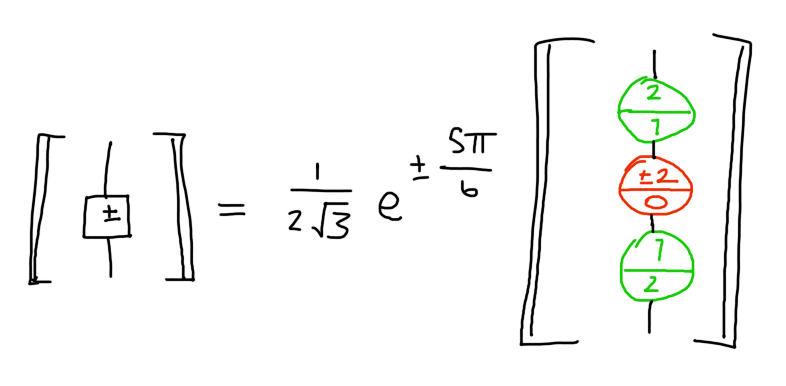
\includegraphics[scale=0.3]{figures/sketches/Qutrit Potts matrices.png}
% % \end{equation}

% For the case $q=4$ we are back again in the usual qubit ZX calculus:
% % \begin{equation}
% % 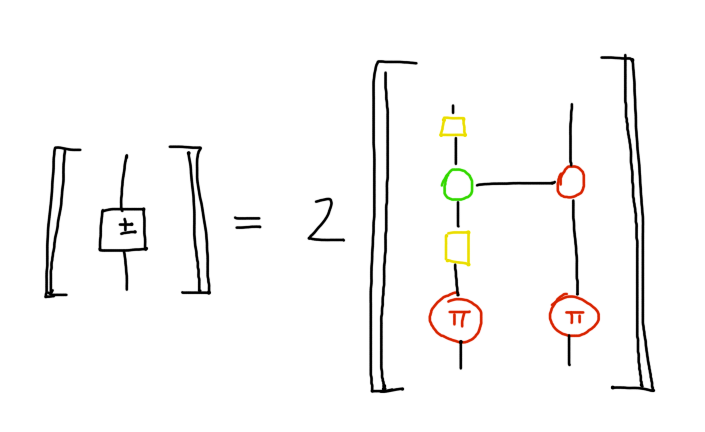
\includegraphics[scale=0.3]{figures/sketches/Qu(4)it Potts matrices.png}
% % \end{equation}

% In each case, the resulting map is in the stabilizer fragment of the ZX calculus. 
 
\section{From a Link to a ZX-Diagram}\label{sec:passage}

We begin by describing the passage from a link $L$ to a ZX-diagram $D$ which represents the evaluation of the Jones polynomial of $L$ at lattice roots of unity. The majority of this journey is as detailed in \citep{jones_tensors}, though the final small step into the ZX-calculus is new. Since this section aims to be comprehensible to those with no background in topology or statistical mechanics, we leave most of the details to \citep{jones_tensors}. We introduce only as many terms as needed to describe the passage fully, keeping definitions simple and providing several figures. After this first jargon-heavy section, we will be working almost exclusively in a ZX setting.\newline

We will define an \textit{n-component link} $L$ to be a smooth embedding of $n$ disjoint circles in $\mathbb{R}^3$. A \textit{link diagram} for $L$ is a projection of the link onto some plane in $\mathbb{R}^3$ but with over- and undercrossing information retained. Thus a given link has infinitely many link diagrams. Intuitively, a link diagram is what one produces when one attempts to draw a link in two dimensions. An \textit{oriented link} has a direction assigned to each component; this is indicated in a link diagram by an arrow. As an example is shown below:\newline

[diagram]\newline

Two oriented links $L$ and $L'$ are isotopic, written $L \simeq L'$, if and only if there is a finite sequence of \textit{Reidemeister moves} [ToDo: ref] taking a diagram for $L$ to a diagram for $L'$. These moves precisely capture the notion of reversible local strand deformations that do not change the topology. For example, they do not permit breaking or gluing of strands, passing one strand through another, or reversing of orientations. The \textit{Jones polynomial} $V_L(z)$ for an oriented link $L$ is a polynomial in $z \in \mathbb{C}$. It is a \textit{link invariant}; that is, $V_L(z) \neq V_{L'}(z)$ implies $L \not\simeq L'$, for any two oriented links $L$ and $L'$. In general, computing $V_L(z)$ is exponentially costly in the number $\abs{C}$ of crossings of $L$, but it is known that at the special cases of the \textit{lattice roots of unity} $z \in \{\pm 1, \pm i, \pm e^{i\frac{2\pi}{3}}, \pm e^{i\frac{4\pi}{3}}\}$ it can be evaluated in time polynomial in $\abs{C}$ [Welsh]:\newline

[Draw lattice roots of unity]\newline

Now, for any diagram of a link $L$ there is an associated \textit{Tait graph}. This is denoted $G_L = (V_L, E_L)$ and obtained as follows. First, the link diagram is given a \textit{checkerboard colouring}. That is, regions of $\mathbb{R}^2$ carved out by the link are shaded black or white such that no two adjacent regions have the same colour. For any diagram for $L$ there are exactly two equivalent ways to do this, the difference between the two just being that the roles of black and white are swapped throughout. Therefore we fix a convention that the unique unbounded region surrounding the link (i.e. the background) will be white.\newline

[diagram]\newline

Next, every shaded (black) region is mapped to a vertex and every crossing is mapped to a signed edge $e = vw$ according the rule shown below. The signs $\varepsilon_{vw} = \pm$ of these edges are called \textit{Tait signs} and are graphically denoted by a small box on the corresponding edge, labelled with either a plus or minus sign appropriately:\newline

[diagram]\newline

If we now suppose that the vertices and Tait signs actually represent \textit{tensors} (multidimensional matrices), then this Tait graph above can be interpreted as a closed \textit{tensor network} in diagrammatic notation [ToDo: ref], which we'll denote $Z(q)$. In fact, suppose we let $z_q = \frac{1}{2}\left(q - 2 + \sqrt{q(q - 4)}\right)$, and let the vertices and Tait signs denote the following tensors:

\begingroup
	\renewcommand*{\arraystretch}{1.25}
	\begin{equation}\label{eq:pm_tensor}
		T_\pm^{(q)} = 
		\left\llbracket \ \tikzfig{pm_maps/pm} \ \right\rrbracket = 
		\begin{pmatrix}
			-z_q^{\mp 1} & 1 & \dots & 1 \\
			1 & -z_q^{\mp 1} & \dots & 1 \\
			\vdots & \vdots & \ddots & \vdots\\
			1 & 1 & \dots & -z_q^{\mp 1}
		\end{pmatrix}
	\end{equation}
	\begin{equation}\label{eq:vertex_tensor}
		\tilde{T}^{(q)} =
		\left\llbracket \ \ \tikzfig{pm_maps/vertex} \ \ \right\rrbracket = 
		\text{ToDo}
	\end{equation}
\endgroup

Then remarkably the resulting closed tensor network $Z(q)$ is equal to the Jones polynomial $V_L(z_q)$ at these specific points, up to a prefactor $\mathcal{A}_L(q)$ [ToDo: ref]. Computing this prefactor is known to be efficient, so if we can show that computing $Z(q)$ is also efficient then we'll have shown that computing $V_L(z_q)$ is efficient. Note the correspondence $(z_1, z_2, z_3, z_4) = (e^{i\frac{2\pi}{3}}, i, e^{i\frac{\pi}{3}}, 1)$ with the lattice roots of unity. 

\begin{remark}
	Of course, different diagrams for $L$ will lead to different (non-isomorphic) Tait graphs $G_L$. Ultimately, however, this will not matter to us. This is because the Tait signs $\varepsilon_{vw}$ are related to $z_q$ in such a way that graph operations on $G_L$ corresponding to Reidemeister moves on $L$ leave $Z(q)$ (ToDo: and $\mathcal{A}_L(q)$?) invariant [ToDo: ref].
\end{remark}

\begin{remark}
	$Z(q)$ is in fact the partition function of a $q$-state Potts model placed on the Tait graph $G_L$. [ToDo: say more?]
\end{remark}

In order to demonstrate efficient computability of $Z(q)$ for $q \in \{1, 2, 3, 4\}$, we will find representations for the tensors $T_\pm^{(q)}$ and $\tilde{T}^{(q)}$ in the \textit{ZX-calculus}, a graphical language for quantum mechanics based on $q$-dimensional qudits, introduced formally in the next two sections. For $q=1$ the calculus is trivial - there is exactly one $1$-dimensional qudit - so only the cases $q \in \{2, 3, 4\}$ remain. For $q=4$ the isomorphism $\mathbb{C}^4 \cong \mathbb{C}^2 \otimes \mathbb{C}^2$ means we can use the same 2-dimensional calculus as for $q=2$. We will soon see that both the 2-dimensional (\textit{qubit}) and 3-dimensional (\textit{qutrit}) ZX-calculus feature \textit{green spiders}, and in all three cases $q \in \{2, 3, 4\}$ these are the right choice of representative of the vertex tensor $\tilde{T}^{(q)}$.

\begin{proposition}\label{prop:vertex_tensor_Z_spider}
	The tensor represented by a vertex in the Tait graph is related (ToDo: how!?) to the \textit{standard interpretation} of the green spider in the cases $q \in \{2, 3, 4\}$.
	\begin{equation*}
		\tilde{T}^{(q)} \ = \ 
		\left\llbracket \ \ \tikzfig{pm_maps/vertex} \ \ \right\rrbracket \ \sim \ 
		\left\llbracket \ \ \tikzfig{pm_maps/z_spider} \ \ \right\rrbracket
	\end{equation*}
	\begin{proof}
		See Appendix [ToDo].
	\end{proof}
\end{proposition}

ZX-diagrams corresponding to the $q \times q$ matrix $T_\pm^{(q)}$ are given after the ZX-calculi have been properly introduced (Propositions \ref{prop:pm_map_q2_q4} and \ref{prop:pm_map_q3}). [ToDo: say more! Move discussion about scalar exactness here? Explain how contracting this tensor network/ZX-diagram means evaluating $Z(q)$?]


% Let $z_q = \frac{1}{2}\left(q - 2 + \sqrt{q(q - 4)}\right)$, and note the correspondence $(z_1, z_2, z_3, z_4) = (e^{i\frac{2\pi}{3}}, i, e^{i\frac{\pi}{3}}, 1)$ with the lattice roots of unity. Remarkably, the Jones polynomial $V_L(z_q)$ at the points $q \in \{1, 2, 3, 4\}$ can be expressed in terms of the \textit{partition function} $Z(q)$ of a \textit{$q$-state Potts model} [Wu]. 



% For those with no statistical mechanical background, given some graph $G = (V, E)$, a $q$-state Potts model on $G$ can just be thought of as the ability to assign a \textit{spin} $\sigma_v \in \{1, ..., q\}$ to each vertex $v \in V$, along with a partition function $Z: \{1, .., q\} \rightarrow \mathbb{C}$, which in physics usually captures some thermodynamical properties of a system. This function has an explicit formula in the general case, but it will make more sense to defer stating this until we have introduced enough terminology to give a simpler formula pertaining to our circumstances (see [ToDo] below). A particular assignment $\sigma = (\sigma_1, ..., \sigma_{\abs{V}})$ of spins to each vertex will be called a \textit{configuration}.\newline

% In our case, we will define a Potts model on a particular \textit{signed graph} - a graph in which every edge has a positive or negative sign - called a \textit{Tait graph} of the link $L$. This is denoted $G_L = (V_L, E_L)$ and obtained as follows. First, an arbitrary link diagram for $L$ is given a \textit{checkerboard colouring}. That is, regions of $\mathbb{R}^2$ carved out by the link are shaded black or white such that no two adjacent regions have the same colour. For any diagram for $L$ there are exactly two equivalent ways to do this, the difference between the two just being that the roles of black and white are swapped throughout. Therefore we fix a convention that the unique unbounded region surrounding the link (i.e. the background) will be white.\newline

% [Diagram]\newline

% Next, every shaded (black) region is mapped to a vertex and every crossing is mapped to a signed edge $e = vw$ according to its orientation relative to the surrounding colours, per the rule shown in [ToDo] below. The signs $\varepsilon_{vw} = \pm$ of these edges are called \textit{Tait signs} and are graphically denoted by a small box on the corresponding edge, labelled with either a plus or minus sign appropriately. If we now define a Potts model on $G_L$, the partition function $Z(q)$ has the following formula. We sum over all possible configurations $\sigma$ of spins, and within each term we multiply together the values $-z_q^{-\varepsilon_{vw}}$ for all edges $vw$ whose endpoints have the same spin in this configuration. That is:

% \begin{equation}
% 	Z(q) = \sum_{\sigma} \left( \prod_{vw \in E_L} T_{\sigma_v, \sigma_w}^{(q)} \right)
% \end{equation}
% \begin{equation}
% 	T_{\sigma_v, \sigma_{w}}^{(q)}
% 	= \begin{cases}
% 		-z_q^{-\varepsilon_{vw}} &\ \ \text{if} \ \ \sigma_v = \sigma_{w} \\  
% 		1 &\ \ \text{if} \ \ \sigma_v \neq \sigma_{w}
% 	\end{cases}
% \end{equation}

% For fixed $v, w$ we can view $T_{(-)_v,(-)_w}^{(q)} \eqdef T_{\varepsilon_{vw}}^{(q)}$ as a $q \times q$ matrix, indexed by the possible spins $\{1, ..., q\}$ that could be assigned to $v$ and $w$: 

% \begingroup
% 	\renewcommand*{\arraystretch}{1.5}
% 	\begin{equation}
% 	T_{-_v,-_w}^{(q)}
% 	\begin{pmatrix}
% 		-z_q^{-\varepsilon_{vw}} & 1 & \dots & 1 \\
% 		1 & -z_q^{-\varepsilon_{vw}} & \dots & 1 \\
% 		\vdots & \vdots & \ddots & \vdots\\
% 		1 & 1  & \dots & -z_q^{-\varepsilon_{vw}}
% 	\end{pmatrix}
% \end{equation}
% \endgroup

% Finally, the actual statement relating the Jones polynomial to the partition function is:

% \begin{equation}
% 	V_L(z_q) = \mathcal{A}_L(q)Z(q)
% \end{equation}

% where $\mathcal{A}_L(q)$ is an efficiently computable prefactor, whose definition is given in Appendix [ToDo]. 
% % For completeness, we give its formula, where $w(L)$ denotes the \textit{writhe} of the link $L$ [ToDo: ref], and the \textit{Tait number} $\tau(L)$ is the sum $\sum_{vw \in E_L} \varepsilon_{vw}$ of all the Tait signs:
% % \begin{equation}
% % 	\mathcal{A}_L(q) = (-z_q^{\frac{1}{2}} - z_q^{-\frac{1}{2}})^{-\abs{V_L} - 1}(-z_q^{\frac{3}{4}})^{w(L)}z_q^{\frac{1}{4}\tau(L)}
% % \end{equation}

% \begin{remark}
% 	Of course, different diagrams for $L$ will lead to different (non-isomorphic) Tait graphs $G_L$. Ultimately, however, this will not matter to us. This is because the Tait signs are related to $z_q$ in such a way that graph operations on $G_L$ corresponding to Reidemeister moves on $L$ leave $Z(q)$ (ToDo: and therefore $\mathcal{A}_L(q)$?) invariant [ToDo: ref].
% 	 % $\varepsilon_{vw} = \pm$ determine \textit{spin-spin interactions} $J_{\pm} = \text{[ToDo]}$, which are related to the variable $z_q$ of the Jones polynomial $V_L(z_q)$ via the equality $z_q = -e^{\mp J_\pm}$. As a result, it can be shown [ToDo ref] that the interactions $J_\pm$ are such that the graph operations on $G_L$ corresponding to Reidemeister moves on $L$ leave $Z(q)$ invariant. 
% \end{remark}



% After defining a Potts model on the Tait graph $G_L$, every signed edge indicates a \textit{spin-spin Tait-sign-dependent interaction} $J_\pm \in \mathbb{C}$. These interactions relate to the variable $z$ of the Jones polynomial via the equality $z = -e^{\mp J_\pm}$. The role of the link invariant is played by the partition function $Z(q)$; in fact, the interactions $J_\pm$ are such that the graph operations on $G_L$ corresponding to Reidemeister moves on $L$ leave $Z(q)$ invariant. Specifically, $Z(q)$ is related to the Jones polynomial by $V_L(z) = \mathcal{A}_L(z)Z(q)$, where $A_L(z)$ is an efficiently computable value which handles bookeeping of twist factors [Definition?]. Its explicit definition is given in [ToDo] in the Appendix. has the following explicit formula: [Check again with Kon!]\newline






% For the case $q=3$ we use the qutrit ZX calculus:
% % \begin{equation}
% % 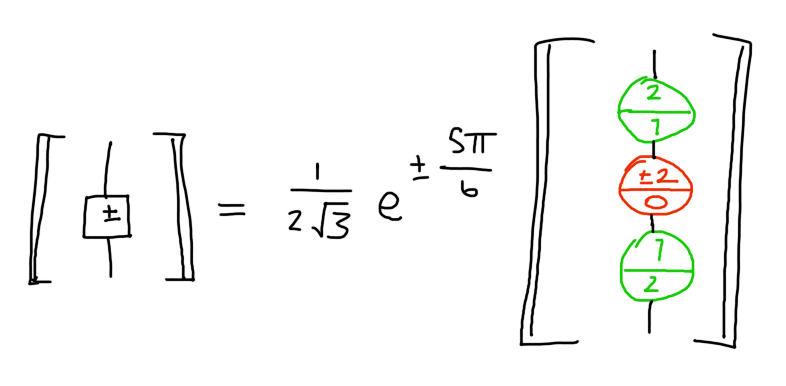
\includegraphics[scale=0.3]{figures/sketches/Qutrit Potts matrices.png}
% % \end{equation}

% For the case $q=4$ we are back again in the usual qubit ZX calculus:
% % \begin{equation}
% % 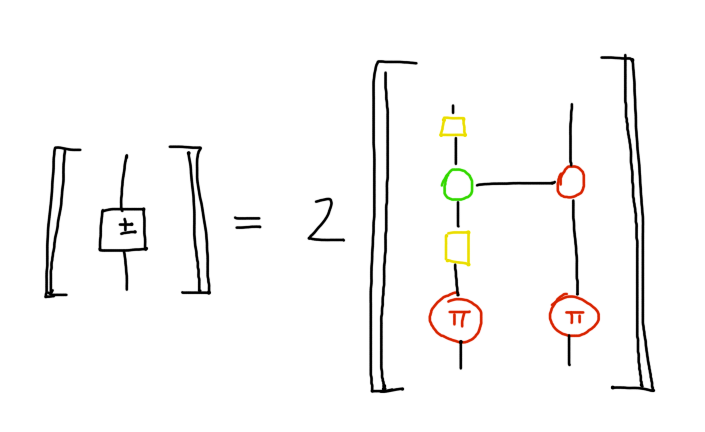
\includegraphics[scale=0.3]{figures/sketches/Qu(4)it Potts matrices.png}
% % \end{equation}

% In each case, the resulting map is in the stabilizer fragment of the ZX calculus. 
 

\section{Simplifying Qubit ZX-Diagrams}

\subsection{The Qubit ZX-Calculus}

Here we give a quick introduction to the qubit ZX-calculus. For a more detailed treatment, see \cite[][Chapter 9.4]{PQP}. The qubit ZX-calculus is a diagrammatic language for quantum mechanics consisting of \textit{spiders} connected together by \textit{wires}, living within a rectangular plane. Diagrams are read bottom-to-top. Wires that don't end at a spider are \textit{inputs} (if their non-spider end starts at the bottom of the plane) and/or \textit{outputs} (if their non-spider end lies at the top of the plane).\newline

Only the topology matters; spiders can move freely around the plane and wires can be deformed and pass over each other, provided the connections between components remain unchanged. The single exception is the endpoints of input and output wires; these are fixed on the boundary of the plane. Spiders come in two species: green $Z$-spiders and red $X$-spiders, decorated by a \textit{phase} angle $\alpha$. When this phase is zero, we will omit it. The diagrammatic formalism exists in the abstract, but we say that it has a \textit{standard linear algebraic interpretation}. 

\begin{definition}\label{def:qubit_standard_spiders}
	Given the usual vectors $\{\ket{0}$, $\ket{1}\}$ (the \textit{$Z$-basis}) and $\{\ket{+}$, $\ket{-}\}$ (the \textit{$X$-basis}) in $\mathbb{C}^2$, the \textit{standard interpretations} of $Z$- and $X$- spiders respectively are:
	\begin{equation*}
		\left\llbracket \ \tikzfig{qubit_spiders/Z_a_labelled} \ \right\rrbracket = 
		\ket{0}^{m}\bra{0}^{n} + 
		e^{i\alpha}\ket{1}^{m}\bra{1}^{n} ,
		\quad
		\left\llbracket \ \tikzfig{qubit_spiders/X_a_labelled} \ \right\rrbracket = 
		\ket{+}^{m}\bra{+}^{n} + 
		e^{i\alpha}\ket{-}^{m}\bra{-}^{n}
	\end{equation*}
\end{definition}

% \begingroup
% 	\allowdisplaybreaks
% 	\setlength{\jot}{10pt}
% 		\begin{align}
% 			&\left\llbracket \ \tikzfig{qubit_spiders/Z_a_labelled} \ \right\rrbracket = 
% 			\ket{0}^{\otimes m}\bra{0}^{\otimes n} + 
% 			e^{i\alpha}\ket{1}^{\otimes m}\bra{1}^{\otimes n} \\
% 			&\left\llbracket \ \tikzfig{qubit_spiders/X_a_labelled} \ \right\rrbracket = 
% 			\ket{+}^{\otimes m}\bra{+}^{\otimes n} + 
% 			e^{i\alpha}\ket{-}^{\otimes m}\bra{-}^{\otimes n}
% 		\end{align}
% \endgroup

Using this standard interpretation, and writing $\simeq$ to mean `equal up to a scalar factor', we can represent common quantum computing concepts as ZX-diagrams. Spiders with one output and no inputs are called \textit{states}, while those with one input and no outputs are called \textit{effects}.

\begin{example}
	The standard interpretations of the diagrams below are as follows:
	\begin{equation}
		\left\llbracket \ \tikzfig{qubit_common/+} \ \right\rrbracket \simeq \ket{+} , \quad
		\left\llbracket \ \tikzfig{qubit_common/1} \ \right\rrbracket \simeq \ket{1} , \quad
		\left\llbracket \ \tikzfig{qubit_common/X_a} \ \right\rrbracket = X_{\alpha} , \quad
		\left\llbracket \ \tikzfig{qubit_common/cnot} \ \right\rrbracket \simeq \text{CNOT}
	\end{equation}
\end{example}

\begin{remark}
	In the ZX-calculus, equality of diagrams translates to equality only up to some scalar factor in the standard linear algebraic interpretation. This has often proved to be more convenient in quantum computing, but for calculating Jones polynomials of knots at lattice roots of unity - which are ultimately just complex numbers - this is manifestly insufficient. However, to simply prove that the calculation of such polynomials is efficient, this suffices - provided we also show that keeping track of the `missing' scalars can be done efficiently. See the end of this section for a discussion of this last point.
\end{remark}

We introduce a small yellow box to denote the Hadamard gate $H$. We will also often omit the yellow box entirely and instead draw a dashed blue line - we call these equivalent diagrams a \textit{Hadamard edge}:

\begin{equation}
	\tikzfig{qubit_hadamard/yellow_box} \quad = \quad
	\tikzfig{qubit_hadamard/dashed} \quad = \quad
	\tikzfig{qubit_hadamard/decomposed}
\end{equation}

The diagrams that can be formed from such spiders and wires are then subject to the rewrite rules in Figure \ref{fig:qubit_ZX_rules}. These rules constitute the definition of the ZX-calculus. Note that due to $\qubitRuleColourChange$ and $\qubitRuleHadamard$ all rules hold with the roles of red and green (i.e. $Z$ and $X$) interchanged.\newline

\begin{figure}
	\begin{tcolorbox}[colback=white]
		\begin{equation*}
		\vspace{-5pt}
			\tikzfig{qubit_rules/fusion/lhs} \ = \ 
			\tikzfig{qubit_rules/fusion/rhs} \quad \hypertarget{qubit_rule_fusion}{\mathbf{(f)}}
			\hspace{50pt}
			\tikzfig{qubit_rules/bialgebra/lhs} \ = \
			\tikzfig{qubit_rules/bialgebra/rhs} \quad \hypertarget{qubit_rule_bialgebra}{\mathbf{(b)}}
		\end{equation*}
		\vspace{5pt}
		\begin{equation*}
			\tikzfig{qubit_rules/identity/lhs} \ = \
			\tikzfig{qubit_rules/identity/rhs} \quad \hypertarget{qubit_rule_id}{\mathbf{(id)}}
			\hspace{50pt}
			\tikzfig{qubit_rules/hadamard/lhs} \ = \
			\tikzfig{qubit_rules/hadamard/rhs} \quad \hypertarget{qubit_rule_hadamard}{\mathbf{(H)}}
			\hspace{50pt}
			\tikzfig{qubit_rules/colour_change/lhs} \ = \
			\tikzfig{qubit_rules/colour_change/rhs} \quad \hypertarget{qubit_rule_colour_change}{\mathbf{(cc)}}
		\end{equation*}
		\vspace{5pt}
		\begin{equation*}
			\tikzfig{qubit_rules/copy/lhs} \ = \ \
			\tikzfig{qubit_rules/copy/rhs} \quad \hypertarget{qubit_rule_copy}{\mathbf{(cp)}}
			\hspace{50pt}
			\tikzfig{qubit_rules/pi/lhs} \ = \
			\tikzfig{qubit_rules/pi/rhs} \quad \hypertarget{qubit_rule_pi}{(\bm{\pi})}
		\end{equation*}
		\vspace{3pt}
	\end{tcolorbox}
	\vspace{5pt}
	\caption{Rewrite rules for the qubit ZX-calculus. The fusion rule $\mathbf{(f)}$ applies to spiders connected by at least one wire.}
	\label{fig:qubit_ZX_rules}
	\vspace{-1pt}
\end{figure}

% \begin{remark}\label{rem:qubit_scalar_exactness} 
% 	A small technical remark is in order: the rule set given here is complete for qubit stabilizer quantum mechanics when equality is taken only up to a scalar factor. To achieve completeness under exact equality, a slighly modified rule set would be required, as in (for example) \citep{backens_scalar_exact}. But for our purposes this would be overkill; in order to show that the Jones polynomial of knots at lattice roots of unity is efficiently computable, it suffices to consider the `non-exact' rules - i.e. it suffices to show such a Jones polynomial is efficiently computable up to a scalar factor. But of course to actually compute such a Jones polynomial, we will need to keep track of scalars.
% \end{remark}

We can now give ZX-diagrams whose standard interpretations are equal (up to a scalar) to the matrices $T_{\pm}^{(q)}$ in \eqref{eq:pm_tensor} for $q \in \{2, 4\}$.

% [Move commented out stuff below to appendix proof?]

% DON"T DELETE!!!!!!!!!!!!!!!!!!!!!!!
 % This is because the standard interpretation of diagrams more complex than a single spider can be derived as follows. First a diagram is divided into horizontal strips, then these strips are themselves divided vertically, so that the diagram consists of spiders composed in parallel (side-by-side, written $\otimes$) and in sequence (on top of each other, with legs fused together, written $\circ$). Such a division always exists, though it may require a diagram deformation. For example:

% For spiders $S$ and $T$, we then have:

% \begin{equation}
% 	\left\llbracket S \otimes T \right\rrbracket = \left\llbracket S \right\rrbracket \otimes \left\llbracket T \right\rrbracket 
% \end{equation} 
% \begin{equation}	
% 	\left\llbracket S \circ T \right\rrbracket = \left\llbracket S \right\rrbracket \left\llbracket T \right\rrbracket 
% \end{equation} 

% where on the right hand side of the first equation the $\otimes$ symbol means the Kronecker product of two matrices. Thus a diagram with standard interpretation $T_{2\pm}$ will have one input and one output, while a diagram for $T_{4\pm}$ will have two inputs and two outputs.

\begin{proposition}\label{prop:pm_map_q2_q4}
	Under the standard interpretation as linear maps, the following diagrams give (up to a scalar) the required matrices:
	\begin{equation}
		\left\llbracket \ \tikzfig{pm_maps/q2} \ \right\rrbracket \simeq \left\llbracket \ \tikzfig{pm_maps/pm} \ \right\rrbracket_{q=2} , 
		\qquad\quad
		\left\llbracket \ \tikzfig{pm_maps/q4} \ \right\rrbracket \simeq \left\llbracket \ \tikzfig{pm_maps/pm} \ \right\rrbracket_{q=4} .
	\end{equation}
	\begin{proof}
		See Appendix \ref{prop:pm_maps_zx_appendix}.
	\end{proof}
\end{proposition}

The \textit{stabilizer fragment} of the calculus consists of all diagrams in which all phases are integer multiples of $\frac{\pi}{2}$. We note that both diagrams above fall into this stabilizer fragment. Now, in \cite[][Theorem 5.4]{graph_theoretic_simplification} the authors give an efficient algorithm for simplifying any qubit ZX-diagram to an equivalent diagram with fewer spiders. In particular, given a stabilizer diagram that is \textit{closed} (has neither inputs nor outputs), the algorithm efficiently simplifies it until it contains at most one spider. If it exists, this spider is green, legless and has phase in $\{0, \pi\}$. We briefly outline the process here, referring the reader to \citep{graph_theoretic_simplification} for a full discussion. First it is shown that every diagram is equivalent to a \textit{graph-like} diagram.

\begin{definition}
	\cite[][Definition 3.1]{graph_theoretic_simplification} A qubit ZX-diagram is \textit{graph-like} when:
	\begin{enumerate}
		\item Every spider is a Z-spider.
		\item Spiders are only connected by Hadamard edges.
		\item There are no parallel Hadamard edges or self-loops.
		\item Every input and output is connected to a spider.
		\item Every spider is connected to at most one input or output.
	\end{enumerate}
\end{definition}

Then the following two results are used to eliminate spiders. For more details on \textit{local complementation} and \textit{pivoting}, see \cite[][Section 4]{graph_theoretic_simplification}. 

\begin{theorem}\label{thm:qubit_eliminate_spiders}
	The following equation holds in the qubit ZX-calculus:
	\begin{equation}\label{eq:eliminate_clifford}
		\tikzfig{eliminate/clifford}
	\end{equation}

	This says we can remove any spider $i$ with phase $\pm\frac{\pi}{2}$, at the cost of performing a local complementation at $i$. Similarly, the following equation holds in the qubit ZX-calculus:

	\begin{equation}\label{eq:eliminate_pauli}
		\tikzfig{eliminate/pauli}
	\end{equation}

	This says we can remove any pair $i, j$ of spiders with phases in $\{0, \pi\}$ connected by a Hadamard edge, at the cost of performing a local pivot along the edge $uv$. 

	\begin{proof}
		These are Lemmas 5.2 and 5.3 in \citep{graph_theoretic_simplification}
	\end{proof}
\end{theorem}

After each application of \eqref{eq:eliminate_clifford} or \eqref{eq:eliminate_pauli}, the following lemma is used to remove any parallel Hadamard edges, and ensure the diagram remains graph-like.

\begin{lemma}\label{lem:2_h_edges_vanish}
	The following result holds in the qubit ZX-calculus:
	\begin{equation}
		\tikzfig{hadamard_lemmas/2_h_edges_vanish/lhs} \quad = \quad \tikzfig{hadamard_lemmas/2_h_edges_vanish/rhs}
	\end{equation}
	\begin{proof}
		This is Equation (3) in \citep{graph_theoretic_simplification}. 
	\end{proof}
\end{lemma}

Since any ZX-diagram derived from a knot in the manner described in Section \ref{sec:passage} will be closed, this algorithm suffices to prove that the calculation of the Jones polynomial of any knot at the lattice roots of unity $\pm 1$ and $\pm i$ is efficient. This is because reading off the scalar at the end is trivial; either we have the empty diagram, which has standard interpretation $1$, or a single legless $Z$-spider with phase $k\pi$:

\begin{equation}
	\left\llbracket \ \tikzfig{scalars/Z_kpi_1} \ \right\rrbracket = 
	\left\llbracket \ \tikzfig{scalars/Z_kpi_2} \ \right\rrbracket = 
	( \bra{0} + \bra{1} )( \ket{0} + e^{ik\pi}\ket{1} ) =
	1 + e^{ik\pi}
\end{equation}

Furthermore, keeping track of the scalar factors introduced with each application of Theorem \ref{thm:qubit_eliminate_spiders} or Lemma \ref{lem:2_h_edges_vanish} can be done efficiently. [ToDo: proof, if not explicitly doing all this in a scalar-exact fashion. Reference Backens]

\section{Simplifying Qutrit ZX-Diagrams}

For the remaining case $q=3$, we will show that we can generalise all the ideas of the previous section to the qutrit ZX-calculus, which we must first define.

\subsection{The Qutrit ZX-Calculus}

[ToDo: make it more bitesize - theorems, definitions, etc?]

As before, this calculus is based around spiders and wires, but there are key differences, some subtler than others. To get a feel for the qutrit calculus, we outline these differences briefly here before giving a formal definition. First of all, the qubit $Z$-basis consisted of two vectors $\ket{0} = \smallcolvec{1\\0}$ and $\ket{1} = \smallcolvec{0\\1}$, whereas the qutrit $Z$-basis consists of three vectors:

\begin{equation}
	\ket{0} = \smallcolvec{1\\0\\0}, \hspace{20pt}
	\ket{1} = \smallcolvec{0\\1\\0}, \hspace{20pt}
	\ket{2} = \smallcolvec{0\\0\\1}. 
\end{equation}
 
Similarly, letting $\omega = e^{\frac{2}{3}\pi i}$, the qutrit $X$-basis consists of the three vectors: 

\begin{align}
	\ket{+} &= \frac{1}{\sqrt{3}} \left(\ket{0} + \ket{1} + \ket{2}\right)\\
	\ket{\omega} &= \frac{1}{\sqrt{3}} \left(\ket{0} + \omega\ket{1} + \bar{\omega}\ket{2}\right)\\
	\ket{\bar{\omega}} &= \frac{1}{\sqrt{3}} \left(\ket{0} + \bar{\omega}\ket{1} + \omega\ket{2}\right)
\end{align}

Spiders thus carry \textit{two} phases $\alpha$ and $\beta$, and have the following standard interpretation as linear maps:

\begingroup
	\allowdisplaybreaks
	\setlength{\jot}{10pt}
		\begin{align}
			&\left\llbracket \quad \tikzfig{qutrit_generators/spiders/Z_a_b_labelled} \quad \right\rrbracket = 
			\ket{0}^{m}\bra{0}^{n} + 
			e^{i\alpha}\ket{1}^{m}\bra{1}^{n} + 
			e^{i\beta}\ket{2}^{m}\bra{2}^{n} \\
			&\left\llbracket \quad \tikzfig{qutrit_generators/spiders/X_a_b_labelled} \quad \right\rrbracket = 
			\ket{+}^{m}\bra{+}^{n} + 
			e^{i\alpha}\ket{\omega}^{m}\bra{\omega}^{n} + 
			e^{i\beta}\ket{\bar{\omega}}^{m}\bra{\bar{\omega}}^{n}
			% &\left\llbracket \quad \tikzfig{qutrit_generators/spiders/Z_a_b_labelled} \quad \right\rrbracket = 
			% \ket{0}^{\otimes m}\bra{0}^{\otimes n} + 
			% e^{i\alpha}\ket{1}^{\otimes m}\bra{1}^{\otimes n} + 
			% e^{i\beta}\ket{2}^{\otimes m}\bra{2}^{\otimes n} \\
			% &\left\llbracket \quad \tikzfig{qutrit_generators/spiders/X_a_b_labelled} \quad \right\rrbracket = 
			% \ket{+}^{\otimes m}\bra{+}^{\otimes n} + 
			% e^{i\alpha}\ket{\omega}^{\otimes m}\bra{\omega}^{\otimes n} + 
			% e^{i\beta}\ket{\bar{\omega}}^{\otimes m}\bra{\bar{\omega}}^{\otimes n}
		\end{align}
\endgroup

When $\alpha = \beta = 0$ we will again omit the angles entirely, and just draw a small green or red dot. 

\begin{warning}
	Throughout, we slightly abuse notation by letting $1$ and $2$ denote the commonly used angles $\frac{2\pi}{3}$ and $\frac{4\pi}{3}$ respectively. This shouldn't ever cause confusion.
\end{warning}

Hadamard boxes change too: they are now neither self-conjugate nor self-adjoint, though they remain self-transpose. Therefore in keeping with the diagrammatic paradigm we ought to stop representing them as boxes, and instead pick something that has neither vertical nor horizontal symmetry, but is invariant under rotation by $\pi$. A parallelogram fits the bill.

\begin{definition}
	In the qutrit ZX-calculus, the \textit{Hadamard edge} (\textit{$H$-edge}) and its adjoint (\textit{$H^\dagger$-edge}) are respectively the two diagrams below. We resurrect the dashed blue line notation from the qubit case, and additionally use a purple dashed line for $H^\dagger$-edges:
	\begin{equation}
		\tikzfig{qutrit_rules/hadamard/euler/h} \ = \ 
		\tikzfig{hadamard_lemmas/dashed/blue} \ = \ 
		\tikzfig{qutrit_rules/hadamard/euler/decomposition} \ , 
		\hspace{75pt}
		\tikzfig{hadamard_lemmas/decompositions/h_dagger} \ = \ 
		\tikzfig{hadamard_lemmas/dashed/purple} \ = \ 
		\tikzfig{hadamard_lemmas/decompositions/h_dagger_zxz}
	\end{equation}
\end{definition}

Now comes the most important difference: in the qutrit ZX-calculus there is no `plain' cap or cup. That is, we have the following two results:

\begin{equation}
	\tikzfig{cups_caps/z_cup} \quad \neq \quad \tikzfig{cups_caps/x_cup} \quad , \hspace{75pt}
	\tikzfig{cups_caps/z_cap} \quad \neq \quad \tikzfig{cups_caps/x_cap}
\end{equation}

This has several consequences. Firstly, the maxim that `only topology matters' no longer applies. That is, it is now important to make clear the distinction between a spider's inputs and outputs, unlike in the qubit case where we could freely interchange the two. Diagram components can still be isotoped around the plane but only so long as this input/output distinction is respected. This gives the qutrit calculus a slightly more rigid flavour than its qubit counterpart. That said, this rigidity is loosened by the following two results: firstly, this distinction is irrelevant for $H$- and $H^\dagger$-edges. 

\begin{lemma}\label{lem:h_edges_input_output}
	In the qutrit ZX-calculus, the following results hold:
	\begin{equation*}
		\tikzfig{hadamard_lemmas/io_irrelevant/h/lhs} \ = \ 
		\tikzfig{hadamard_lemmas/io_irrelevant/h/rhs} \ ,
		\hspace{50pt}
		\tikzfig{hadamard_lemmas/io_irrelevant/h_dagger/lhs} \ = \ 
		\tikzfig{hadamard_lemmas/io_irrelevant/h_dagger/rhs}
	\end{equation*}
	\begin{proof}
		These are Lemmas 3.2 and 3.3 in \citep{qutrit_euler}.
	\end{proof}
\end{lemma}

Secondly, the `snake equations' continue to hold in some form; given a cap and cup of different colours, we can still straighten out the wire between them as before, only now it comes at the cost of adding two Hadamard boxes to the wire. For a cup and cap of the same colour, we can straighten out the wire as usual.

\begin{lemma}
	In the qutrit ZX-calculus, the following results hold. Moreover, they hold with the roles of green and red interchanged. 
	\begin{equation}
		\tikzfig{qutrit_snake/same_bent} \quad = \quad \tikzfig{qutrit_snake/same_straight} \quad ,
		\hspace{50pt}
		\tikzfig{qutrit_snake/different_bent} \quad = \quad \tikzfig{qutrit_snake/different_straight} \quad .
	\end{equation}
	\begin{proof}
		As we will soon see, these are just rules $\qutritRuleFusion$ and $\qutritRuleSnake$.
	\end{proof}
\end{lemma}

We now give a full set of rules defining the qutrit ZX-calculus. Our presentation aims for clarity and accessibility; for a more rigourous description, see \citep{harny_completeness}.

\begin{figure}
	\begin{tcolorbox}[colback=white]
		\begin{equation*}
			% \tikzfig{qutrit_rules/fusion/lhs} \quad = \quad 
			% \tikzfig{qutrit_rules/fusion/middle} \quad = \quad 
			% \tikzfig{qutrit_rules/fusion/rhs} \quad \hypertarget{qutrit_rule_fusion}{\mathbf{(f)}}
			\tikzfig{qutrit_rules/fusion/all} \quad \hypertarget{qutrit_rule_fusion}{\mathbf{(f)}}
		\end{equation*}
		% \vspace{5pt}
		\begin{equation*}
			\tikzfig{qutrit_rules/identity/lhs} \quad = \quad 
			\tikzfig{qutrit_rules/identity/rhs} \quad \hypertarget{qutrit_rule_id}{\mathbf{(id)}}
			\hspace{60pt}
			\tikzfig{qutrit_rules/twisted_cup/lhs} \quad = \quad 
			\tikzfig{qutrit_rules/twisted_cup/rhs} \quad \hypertarget{qutrit_rule_twisted_cup}{\mathbf{(t)}}
		\end{equation*}
		\vspace{5pt}
		\begin{equation*}
			\tikzfig{qutrit_rules/0_copy/lhs} \quad = \quad 
			\tikzfig{qutrit_rules/0_copy/rhs} \quad \hypertarget{qutrit_rule_0_copy}{\mathbf{(cp_0)}}
			\hspace{60pt}
			\tikzfig{qutrit_rules/bialgebra/lhs} \quad = \quad 
			\tikzfig{qutrit_rules/bialgebra/rhs} \quad \hypertarget{qutrit_rule_bialgebra}{\mathbf{(b)}}
		\end{equation*}
		\vspace{5pt}
		\begin{equation*}
			\tikzfig{qutrit_rules/m_copy/1_2_lhs} \quad = \quad 
			\tikzfig{qutrit_rules/m_copy/1_2_rhs} \quad \hypertarget{qutrit_rule_m_copy}{\mathbf{(cp_{\mathcal{M}})}}
			\hspace{60pt}
			\tikzfig{qutrit_rules/m_copy/2_1_lhs} \quad = \quad 
			\tikzfig{qutrit_rules/m_copy/2_1_rhs} \quad \mathbf{(cp_{\mathcal{M}})}
		\end{equation*}
		\vspace{5pt}
		\begin{equation*}
			\tikzfig{qutrit_rules/commute/1_2_lhs} \quad = \quad 
			\tikzfig{qutrit_rules/commute/1_2_rhs} \quad \hypertarget{qutrit_rule_commute}{\mathbf{(cm)}}
			\hspace{60pt}
			\tikzfig{qutrit_rules/commute/2_1_lhs} \quad = \quad 
			\tikzfig{qutrit_rules/commute/2_1_rhs} \quad {\mathbf{(cm)}}
		\end{equation*}
		% \vspace{5pt}
		\begin{equation*}
			\tikzfig{qutrit_rules/hadamard/h_hdagger} \quad = \quad 
			\tikzfig{qutrit_rules/hadamard/identity} \quad = \quad 
			\tikzfig{qutrit_rules/hadamard/hdagger_h} \quad \hypertarget{qutrit_rule_hadamard}{\mathbf{(H)}}
			\hspace{60pt}
			\tikzfig{qutrit_rules/hadamard/euler/h} \quad = \quad 
			\tikzfig{qutrit_rules/hadamard/euler/decomposition} \quad \hypertarget{qutrit_rule_euler}{\mathbf{(E)}}
		\end{equation*}
		% \vspace{5pt}
		\begin{equation*}
			\tikzfig{qutrit_rules/colour_change/lhs} \quad = \quad 
			\tikzfig{qutrit_rules/colour_change/rhs} \quad \hypertarget{qutrit_rule_colour_change}{\mathbf{(cc)}}
			\hspace{60pt}
			\tikzfig{qutrit_rules/colour_change/flip_lhs} \quad = \quad 
			\tikzfig{qutrit_rules/colour_change/flip_rhs} \quad \mathbf{(cc)}
		\end{equation*}
		\vspace{5pt}
		\begin{equation*}
			\tikzfig{qutrit_rules/snake/snake} \quad = \quad 
			\tikzfig{qutrit_rules/snake/hopf_ish} \quad = \quad 
			\tikzfig{qutrit_rules/snake/hadamards} \quad = \quad 
			\tikzfig{qutrit_rules/snake/hadamard_adjoints} \quad \hypertarget{qutrit_rule_snake}{\mathbf{(s)}}
		\end{equation*}
	\end{tcolorbox}
	\vspace{5pt}
	\caption{Rewrite rules for the qutrit ZX-calculus.}
	\label{fig:qutrit_ZX_rules}
\end{figure}

\begin{definition}\label{def:qutrit_ZX_rules}
	The \textit{qutrit ZX-calculus} is a graphical calculus generated by the following diagrams, where $\alpha, \beta \in [0, 2 \pi]$:

	\begin{equation}
		\tikzfig{qutrit_generators/spiders/Z_a_b} \quad , \qquad 
		\tikzfig{qutrit_generators/spiders/X_a_b} \quad , \qquad
		\tikzfig{qutrit_generators/hadamard} \quad , \qquad
		\tikzfig{qutrit_generators/swap} \quad , \qquad
		\tikzfig{qutrit_generators/identity}
	\end{equation}

	and their adjoints $(-)^\dagger$. The non-spider generators' adjoints are their vertical reflections, whereas spiders' adjoints are found by swapping inputs and outputs and negating angles: 

	\begin{equation}
		\left(\ \tikzfig{qutrit_generators/spiders/Z_a_b_labelled}\ \right)^\dagger = \tikzfig{qutrit_generators/spiders/Z_a_b_adjoint_labelled} \quad , \qquad 
		\left(\ \tikzfig{qutrit_generators/spiders/X_a_b_labelled}\ \right)^\dagger = \tikzfig{qutrit_generators/spiders/X_a_b_adjoint_labelled}
	\end{equation}

	These generators can be composed in parallel ($\otimes$) and sequentially ($\circ$), and the resulting diagrams are governed by the rewrite rules in Figure \ref{fig:qutrit_ZX_rules}, wherein addition is modulo $2\pi$. The fusion rule $\qutritRuleFusion$ applies to spiders of the same colour connected by at least one wire. Importantly, all the rules hold under taking adjoints, where for diagrams $D$ and $E$ we have:

	\begin{equation}
		(D \otimes E)^\dagger = D^\dagger \otimes E^\dagger
	\end{equation}
	\begin{equation}
		(D \circ E)^\dagger = D^\dagger \circ E^\dagger
	\end{equation}

	Furthermore, all but the commutation equations $\qutritRuleCommute$ and the colour change equations $\qutritRuleColourChange$ continue to hold when the roles of green and red (i.e. $Z$ and $X$) are interchanged. For these four exceptions, however, analogous equations can be derived from the existing ones; for example, the corresponding colour change equations will be relevant for us later.
\end{definition}
	
\begin{proposition}
	The following equations are derivable in the qutrit ZX-calculus:
	\begin{equation}\label{eq:derived_colour_change}
		\tikzfig{qutrit_rules/exceptions/colour_change/rhs} \quad = \quad \tikzfig{qutrit_rules/exceptions/colour_change/lhs}
		\quad , \qquad
		\tikzfig{qutrit_rules/exceptions/colour_change/flip_rhs} \quad = \quad \tikzfig{qutrit_rules/exceptions/colour_change/flip_lhs}
	\end{equation}
	\begin{proof}
		Add $H$- and $H^\dagger$-boxes to both sides of the original colour change equations in such a way that we can then cancel Hadamards on the legs of the red spiders via $\qutritRuleHadamard$.
	\end{proof}
\end{proposition}

Having now defined the qutrit ZX-calculus we turn our attention back to our tensor network for the Jones polynomial of a knot (ToDo: ref). We are seeking a diagram in the qutrit ZX-calculus that equals (up to a scalar) the matrix $T_{\pm}^{(q)}$ from \eqref{eq:pm_tensor}.

% where we have used $t = \frac{1}{2}(3 - 2 + \sqrt{3(3-4)}) = e^{i\frac{\pi}{3}}$ as in (ToDo: ref). 

\begin{proposition}\label{prop:pm_map_q3}
	Under the standard interpretation as a linear map, the following diagram gives (up to a scalar) the required matrix:
	\begin{equation}
		\left\llbracket \quad \tikzfig{pm_maps/q3} \quad \right\rrbracket \simeq
		% 2\sqrt{3}e^{\mp i\frac{5\pi}{6}} \ 
		\left\llbracket \quad \tikzfig{pm_maps/pm} \quad \right\rrbracket_{q=3} = 
		\begin{pmatrix}
			e^{\mp i\frac{\pi}{3}} & 1 & 1 \\
			1 & e^{\mp i\frac{\pi}{3}} & 1 \\
			1 & 1 & e^{\mp i\frac{\pi}{3}} \\
		\end{pmatrix}
	\end{equation}

	\begin{proof}
		See Appendix \ref{prop:pm_maps_zx_appendix}.
	\end{proof}
\end{proposition}

Crucially, the ZX-diagram in Proposition \ref{prop:pm_map_q3} above is a \textit{stabilizer diagram} in the qutrit ZX-calculus - that is, all angles are integer multiples of $\frac{2\pi}{3}$. Therefore if we can find an algorithm analogous to \cite[][Theorem 5.4]{graph_theoretic_simplification} that efficiently reduces any stabilizer diagram to a trivial one, then we will have shown that the Jones polynomial of any knot at the lattice roots of unity $\pm e^{i\frac{\pi}{3}}$ is efficiently computable. [ToDo: justify the $\pm$]. In the next subsection, we will do exactly that.

% Again - just like in Remark~\ref{rem:qubit_scalar_exactness} - these rules are complete for qutrit stabilizer quantum mechanics when equality is considered only up to a scalar factor; we give the scalar-exact versions (detailed in \citep{qutrit_exact}) so that we can actually compute Jones polynomials later. 


\subsection{Graph-Like Qutrit ZX Diagrams}

% \numbered{Definition}{A \textit{Hadamard edge} (or \textit{H-edge}) is a Hadamard map connecting two spiders. A \textit{Hadamard adjoint edge} (or \textit{$H^\dagger$-edge) }}

[Make all of the following scalar-exact (?)]\newline

We first define a graph-like diagram in the qutrit ZX calculus.

% \numbered{Definition}{A qutrit ZX diagram is \textit{graph-like} when:}
\begin{definition}\label{def:graph_like_qutrit}
	A qutrit ZX-diagram is \textit{graph-like} when: 
	\begin{enumerate}
		\item Every spider is a Z-spider.
		\item Spiders are only connected by Hadamard edges ($H$-edges) or their adjoints ($H^\dagger$-edges).
		\item Every pair of spiders is connected by at most one $H$-edge or $H^\dagger$-edge.
		\item Every input and output is connected to a spider.
		\item Every spider is connected to at most one input or output.
	\end{enumerate}
\end{definition}

Thanks to Lemma \ref{lem:h_edges_input_output} we can ignore which of a spider's $H$- and $H^\dagger$-legs are inputs and outputs. For our specific needs, the last two items above will not be relevant, since ZX-diagrams arising from knots will be closed, but we include them to keep the definition consistent with the qubit case. However, note the difference compared to the qubit case: we need not worry about self-loops beacuse the qutrit ZX calculus doesn't define a `plain' cap or cup. But this comes at a cost: spiders in the qutrit case fuse more fussily. Specifically, when two spiders of the same colour are connected by at least one plain edge and at least one $H$- or $H^\dagger$-edge, fusion is not possible. The following equation, which holds with the roles of $H$ and $H^\dagger$ reversed, helps us get around this:

\begin{equation}\label{eq:spiders_reluctant_to_fuse}
	\tikzfig{hadamard_lemmas/spiders_reluctant_to_fuse/1} \ \xeq{\qutritRuleHadamard} \
	\tikzfig{hadamard_lemmas/spiders_reluctant_to_fuse/2} \ \xeq{\qutritRuleId} \
	\tikzfig{hadamard_lemmas/spiders_reluctant_to_fuse/3}
\end{equation}

We will shortly show that every qutrit ZX-diagram is equivalent to a graph-like one, making use of the following lemmas:

\begin{lemma}\label{lem:three_H_edges_vanish}
	The following equation holds in the qutrit ZX-calculus. Moreover, it holds with the roles of $H$ and $H^\dagger$ interchanged:
	\begin{equation}
		\tikzfig{hadamard_lemmas/3_h_edges_vanish/lhs} \quad = \quad \tikzfig{hadamard_lemmas/3_h_edges_vanish/rhs}
	\end{equation}
	\begin{proof}
		It is shown in~\cite[][Lemma 2.8]{qutrit_euler} that the qutrit ZX-calculus satisfies the following `Hopf law':
		\begin{equation}\label{eq:qutrit_hopf}
			\tikzfig{hadamard_lemmas/3_h_edges_vanish/hopf_law}
		\end{equation}
		Therefore we can argue as follows:
		\begin{equation}
			\tikzfig{hadamard_lemmas/3_h_edges_vanish/lhs} \quad \xeq{\qutritRuleHadamard} \quad
			\tikzfig{hadamard_lemmas/3_h_edges_vanish/step_1} \quad \xeq{\qutritRuleColourChange} \quad
			\tikzfig{hadamard_lemmas/3_h_edges_vanish/step_2} \quad \xeq{\eqref{eq:qutrit_hopf}} \quad
			\tikzfig{hadamard_lemmas/3_h_edges_vanish/step_3} \quad \xeq{\eqref{eq:derived_colour_change}} \quad
			\tikzfig{hadamard_lemmas/3_h_edges_vanish/rhs}
		\end{equation}
	\end{proof}
\end{lemma}

\begin{lemma}\label{lem:H_edges_qutrit} 
	The following two equations hold in the qutrit ZX-calculus. Moreover, they hold with the roles of $H$ and $H^\dagger$ interchanged:
	\begin{equation}
		\tikzfig{hadamard_lemmas/2_h_edges_flip}
		\hspace{75pt}
		\tikzfig{hadamard_lemmas/h_edge_and_adjoint_permute}
	\end{equation}
	\begin{proof}
		This is Lemma 3.4 in\ \cite{qutrit_euler}.
	\end{proof}
\end{lemma}

As we will formalise later, the lemmas above say that we can think of Hadamard edges as $1$-weighted edges and their adjoints as $2$-weighted edges, then work modulo $3$, since every triple of parallel edges disappears. This motivates defining `parametrised' Hadamard gates, which will come in use later:

\begin{equation}
	\tikzfig{hadamard_lemmas/parametrised/0}
	\hspace{75pt}
	\tikzfig{hadamard_lemmas/parametrised/1}
	\hspace{75pt}
	\tikzfig{hadamard_lemmas/parametrised/2}
\end{equation}

The first equation above just says that a `$0$-Hadamard edge' is in fact the empty diagram, and not an edge at all. Where the previous lemmas relate single $H$- and $H^\dagger$-boxes across multiple edges, the next relates multiple $H$- and $H^\dagger$- boxes on single edges.

\begin{lemma}\label{lem:H_boxes_qutrit} 
	The following three equations hold in the qutrit ZX calculus. Moreover, they hold with the roles of $H$ and $H^\dagger$ interchanged:
	\begin{equation}
		\tikzfig{hadamard_lemmas/4_h_boxes_vanish}
		\hspace{75pt}
		\tikzfig{hadamard_lemmas/3_h_boxes_flip}
		\hspace{75pt}
		\tikzfig{hadamard_lemmas/2_h_boxes_separate}
	\end{equation}
	\begin{proof}
		For the first equation, turn the top two $H$-boxes into $H^\dagger$-boxes via $\qutritRuleSnake$, then cancel twice via $\qutritRuleHadamard$. Similarly, for the second equation turn the top two $H$-boxes into $H^\dagger$-boxes via $\qutritRuleSnake$, then cancel once via $\qutritRuleHadamard$, leaving a single $H^\dagger$-box. The third equation is just a simple application of $\qutritRuleId$. Analogous reasoning applies when the roles of $H$ and $H^\dagger$ are swapped.
	\end{proof}
\end{lemma}

Again, intuitively we can think of Hadamard boxes of having value $1$ and their adjoints $-1$ and then work modulo $4$.

\begin{corollary}\label{prop:every_diagram_is_graph_like_qutrit}
	Every qutrit ZX diagram is equivalent to one that is graph-like.
	\begin{proof}
		First use the colour change rule to turn all X-spiders into Z-spiders. Then use Lemma \ref{lem:H_boxes_qutrit} to remove excess $H$- and $H^\dagger$-boxes, inserting a spider between any remaining consecutive pair of such boxes, so that all spiders are connected only by plain edges, $H$-edges or $H^\dagger$-edges. Fuse together as many as possible, and apply \eqref{eq:spiders_reluctant_to_fuse} where fusion is not possible, so that no plain edge connects two spiders. Apply Lemmas \ref{lem:three_H_edges_vanish} and \ref{lem:H_edges_qutrit} to all connected pairs of spiders until at most one $H$- or $H^\dagger$-edge remains between them. Finally, to ensure every input and output is connected to a spider and every spider is connected to at most one input or output, we can use $\qutritRuleHadamard$ and $\qutritRuleId$ to add a few spiders, $H$- and $H^\dagger$-boxes as needed: 
		\begin{equation}
			\tikzfig{is_graph_like/plain_input_output_wire}
			\hspace{75pt}
			\tikzfig{is_graph_like/input_connected_to_hadamard}
			\hspace{75pt}
			\tikzfig{is_graph_like/multiple_inputs_connected_to_one_spider}
		\end{equation}
	\end{proof}
\end{corollary}

\begin{definition}\label{def:graph_state_qutrit}
	A graph-like qutrit ZX diagram is a \textit{graph state} when every spider has zero phase (top and bottom) and is connected to an output. 
\end{definition}

A graph state is described fully by its underlying multigraph, or equivalently by an adjacency matrix, where edges take weights in $\mathbb{Z}_3$\ \cite[][Lemma 4.2]{harny_completeness}. Nodes correspond to phaseless green spiders, edges of weight $1$ correspond to Hadamard edges, and edges of weight $2$ correspond to $H^\dagger$ edges. As in the qubit case, graph states admit a local complementation operation\ \cite[][Definition 2.6]{harny_completeness}, though the effect is now slightly more complicated. We'll give the intuition after the formal definition:

\begin{definition}\label{def:local_complementation_qutrit}
	Given $a \in \mathbb{Z}_3$ and a graph state $G$ with adjacency matrix $W = (w_{i,j})$, the \textit{$a$-local complentation} at node $k$ is the new graph state $G *_a i$, whose adjacency matrix $W' = (w'_{i,j})$ given by:
	\begin{equation}
		w'_{i,j} = w_{i,j} + aw_{i,k}w_{j,k}
	\end{equation}
\end{definition}

So only those edges between neighbours of node $k$ are affected, but rather than just having their weight increased by $1$ (modulo $2$) as in the qubit case, the increase in weight also depends on the weights of the edges from $i$ and $j$ to $k$. As always, this is best seen graphically. For two nodes $i$ and $j$ both connected to $k$ by the same colour edge, $a$-local complementation at $k$ increases weight $w_{i,j}$ by $a$. If instead $i$ and $j$ are connected to $k$ by edges of different colour, $a$-local complementation at $k$ decreases $w_{i,j}$ by $a$. We show a fragment of a ZX-diagram below under the effect of this operation:

\begin{equation}
	\tikzfig{a_local_comp/same}
	\hspace{75pt}
	\tikzfig{a_local_comp/different}
\end{equation}

But the fragment above doesn't give the full picture. As in the qubit case, local complementation gives an equality up to introducing some single qubit phase gates on the outputs.

\begin{theorem}\label{thm:local_comp_equality}
	Given $a \in \mathbb{Z}_3$ and a graph state $(G, W)$ containing a node $k$, let $N(k)$ denote the neighbours of $k$ - that is, nodes $i$ with weight $w_{i,k} \in \{1, 2\}$. Then the following equality holds:
	\ctikzfig{graph_state/local_comp}
	\begin{proof}
		This is Theorem 4.4 and Corollary 4.5 in\ \cite[][]{harny_completeness}.
	\end{proof}
\end{theorem}

Composing local complementations gives a local pivot operation.

\begin{definition}\label{def:local_pivot_qutrit}
	Given $a,b,c \in \mathbb{Z}_3$ and a graph state $G$ containing nodes $i$ and $j$, the \textit{$(a,b,c)$-local pivot} along $ij$ is the new graph state $G \wedge_{(a,b,c)} ij \defeq ((G *_a i) *_b j) *_c i$. 
\end{definition}

This again results in an equality, up to introducing some extra gates on outputs. Here we shall only consider an $(a,-a,a)$-local pivot along an edge $ij$ of non-zero weight, for $a \in \{1, 2\}$. We will call this a \textit{proper $a$-local pivot} along $ij$, and denote it $G \wedge_a ij$.

\begin{theorem}\label{thm:local_pivot_equality}
	Given $a \in \mathbb{Z}_3$ and a graph state $(G, W)$ containing connected nodes $i$ and $j$, define the following:
	\begin{itemize}
		\item $N_{=}(i, j) \defeq \left\{k \in N(i) \cap N(j) \mid w_{k,i} = w_{k,j} \right\}$
		\item $N_{\neq}(i, j) \defeq \left\{k \in N(i) \cap N(j) \mid w_{k,i} \neq w_{k,j} \right\}$
	\end{itemize} 
	Then the following equation relates $G$ and its proper $a$-local pivot along $ij$:
	\ctikzfig{graph_state/proper_local_pivot}

	\begin{proof}
		See Appendix \ref{thm:local_pivot_equality_appendix}.
	\end{proof}
\end{theorem}

These two operations are again the drivers behind the simplification procedure. We classify spiders into three families:

\begin{equation*}
	\mathcal{M} = \left\{\qutritZspider{0}{0}, \qutritZspider{1}{2}, \qutritZspider{2}{1}\right\},
	\hspace{10pt}
	\mathcal{N} = \left\{\qutritZspider{0}{1}, \qutritZspider{1}{0}, \qutritZspider{0}{2}, \qutritZspider{2}{0}\right\},
	\hspace{10pt}
	\mathcal{P} = \left\{\qutritZspider{1}{1}, \qutritZspider{2}{2}\right\}.
\end{equation*}

 exactly as in~\cite[][Theorem 3.1]{harny_completeness}. We call a spider in a graph-like ZX-diagram \textit{interior} if it isn't connected to an input or output (so for our use case all spiders are interior). Given any graph-like ZX-diagram, we will show that we can eliminate pairs of connected interior \Mspiders\ by local pivoting, and standalone interior $\mathcal{N}$- and \Pspiders\ by local complementation.

\begin{theorem}\label{thm:eliminate_M_spiders}
	Given any graph-like ZX-diagram containing two interior \Mspiders\ $i$ and $j$ connected by edge $ij$ of weight $w_{i,j} \eqdef w \in \{1,2\}$, suppose we perform a proper $\pm w$-local pivot along $ij$. Then the new ZX-diagram is related to the old one by the equality:
	
	\ctikzfig{eliminate/M_spiders/theorem_LHS}
	\ctikzfig{eliminate/M_spiders/theorem_RHS}
	
	where all changes to weights of edges where neither endpoint is $i$ or $j$ are omitted. Furthermore, in order to save space, each node with phase \qutritZphase{a_x^y}{b_x^y} is representative of \textit{all} nodes connected to $i$ by an $x$-weighted edge and to $j$ by a $y$-weighted edge.

	\begin{proof}
		See \ref{thm:eliminate_M_spiders_appendix} in the Appendix.
	\end{proof}
\end{theorem}

\begin{theorem}\label{thm:eliminate_N_spiders}
	Given any graph-like ZX-diagram containing an interior \Nspider\ $k$ with phase \qutritZphase{0}{n} for $n \in \{1,2\}$, suppose we perform a $(-n)$-local complementation at $k$. Then the new ZX-diagram is related to the old one by the equality:

	\begin{equation*}
		\tikzfig{eliminate/N_spiders/0_n/step_1} \quad = \quad \tikzfig{eliminate/N_spiders/0_n/step_9}
	\end{equation*}

	where all changes to weights of edges where neither endpoint is $k$ are omitted. If instead $k$ has phase \qutritZphase{n}{0} for $n \in \{1,2\}$, suppose we perform the same $(-n)$-local complementation at $k$. Then the equality relating the new and old diagrams becomes:

	% Spiders with phases \qutritZphase{a_1}{b_1} ... \qutritZphase{a_r}{b_r} are all the neighbours of $k$ connected by a $1$-weighted (blue) edge, while spider with phases \qutritZphase{c_1}{d_1} ... \qutritZphase{c_s}{d_s} are all the neighbours of $k$ connected by a $2$-weighted (purple) edge.\newline

	\begin{equation*}
		\tikzfig{eliminate/N_spiders/n_0/step_1} \quad = \quad \tikzfig{eliminate/N_spiders/n_0/step_9}
	\end{equation*}

	\begin{proof}
		See Appendix \ref{thm:eliminate_N_spiders_appendix}.
	\end{proof}
\end{theorem}

\begin{theorem}\label{thm:eliminate_P_spiders}
	Given any graph-like ZX-diagram containing an interior \Pspider\ $k$ with phase \qutritZphase{p}{p} for $p \in \{1,2\}$, suppose we perform a $p$-local complementation at $k$. Then the new ZX-diagram is related to the old one by the equality:

	\begin{equation*}
		\tikzfig{eliminate/P_spiders/step_1} \quad = \quad \tikzfig{eliminate/P_spiders/step_9}
	\end{equation*}

	where all changes to weights of edges where neither endpoint is $k$ are omitted.

	\begin{proof}
		See Appendix \ref{thm:eliminate_P_spiders_appendix}.
	\end{proof} 

	% Spiders with phases \qutritZphase{a_1}{b_1} ... \qutritZphase{a_r}{b_r} are all the neighbours of $k$ connected by a $1$-weighted (blue) edge, while spider with phases \qutritZphase{c_1}{d_1} ... \qutritZphase{c_s}{d_s} are all the neighbours of $k$ connected by a $2$-weighted (purple) edge.\newline
\end{theorem}

We can now combine these three elimination theorems into an algorithm for efficiently simplifying a closed graph-like ZX-diagram. First note that after applying any one of the three elimination theorems to such a diagram we may end up with a state that is no longer graph-like. Fortunately the only way in which this can happen is if two spiders end up being connected by multiple $H$- or $H^\dagger$-edges, and we have shown via Lemmas \ref{lem:three_H_edges_vanish} and \ref{lem:H_edges_qutrit} that these can always be reduced to just one edge.

\begin{theorem}\label{thm:simplification_algorithm_works}
	Given any closed graph-like ZX-diagram, the following algorithm will always terminate after a finite number of steps, returning an equivalent graph-like ZX-diagram with no \Nspiders, \Pspiders, or adjacent pairs of \Mspiders. Repeat the steps below until no rule matches. After each step, apply Lemmas \ref{lem:three_H_edges_vanish} and \ref{lem:H_edges_qutrit} as needed until the resulting diagram is graph-like:
	\begin{enumerate}
		\item Eliminate an \Nspider\ via Theorem~\ref{thm:eliminate_N_spiders}.
		\item Eliminate a \Pspider\ via Theorem~\ref{thm:eliminate_P_spiders}.
		\item Eliminate two adjacent \Mspiders\ via Theorem~\ref{thm:eliminate_M_spiders}.
	\end{enumerate}
	\begin{proof}
		At every step the total number of spiders decreases by at least one, so since we start with a finite diagram the algorithm terminates after a finite number of steps. By construction, when it does so we are left with an equivalent graph-like ZX-diagram with no \Nspiders, \Pspiders, or adjacent pairs of \Mspiders.
	\end{proof}
\end{theorem}

\begin{corollary}\label{cor:stabilizer_simplification_algorithm_works}
	In particular, if we start with a stabilizer diagram, we can eliminate all but perhaps one \Mspider, depending on whether the initial number of \Mspiders\ was odd or even. 
	\begin{proof}
		No step introduces any non-stabilizer phases.
	\end{proof}
\end{corollary}

The algorithm above could be extended to graph-like diagrams with inputs or outputs as in \cite[][Theorem 5.4]{graph_theoretic_simplification}, but since for our purposes we don't need to do so, we have not gone to the trouble.

\bibliography{ZX-Jones}

\appendix
\section{Appendix}

We begin with proofs of the translations of the matrix $T_{\pm}^{(q)}$ into the ZX-calculus. 

\begin{proposition}\label{prop:pm_maps_zx_appendix} \textbf{/\ Propositions~\ref{prop:pm_map_q2_q4}, \ref{prop:pm_map_q3}.}
	The following equalities hold up to a scalar under the standard interpretation:
	\begin{equation*}
		\left\llbracket \ \tikzfig{pm_maps/q2} \ \right\rrbracket \simeq \left\llbracket \ \tikzfig{pm_maps/pm} \ \right\rrbracket_{q=2} \ , \qquad
		\left\llbracket \ \tikzfig{pm_maps/q3} \ \right\rrbracket \simeq \left\llbracket \ \tikzfig{pm_maps/pm} \ \right\rrbracket_{q=3} \ , \quad
		\left\llbracket \ \tikzfig{pm_maps/q4} \ \right\rrbracket \simeq \left\llbracket \ \tikzfig{pm_maps/pm} \ \right\rrbracket_{q=4}
	\end{equation*}

	\begin{proof}
		Recalling $\omega = e^{i\frac{2\pi}{3}}$, the standard interpretations of phase gates in matrix form are:
		
		\begin{equation*}
			\left\llbracket \ \tikzfig{pm_maps/qubit/Z_phase} \ \right\rrbracket = 
			\begin{pmatrix}
				1 & 0 \\
				0 & e^{i\alpha}
			\end{pmatrix} \ , \quad
			\left\llbracket \ \tikzfig{pm_maps/qubit/X_phase} \ \right\rrbracket = 
			\frac{1}{2} \begin{pmatrix}
				1 + e^{i\alpha} & 1 - e^{i\alpha} \\
				1 - e^{i\alpha} & 1 + e^{i\alpha}
			\end{pmatrix} \ , \quad
			\left\llbracket \ \tikzfig{pm_maps/qutrit/Z_phase} \ \right\rrbracket = 
			\begin{pmatrix}
				1 & 0 & 0\\
				0 & e^{i\alpha} & 0 \\
				0 & 0 & e^{i\beta}
			\end{pmatrix}
		\end{equation*}
		\begin{equation*}
			\left\llbracket \ \tikzfig{pm_maps/qutrit/X_phase} \ \right\rrbracket = 
			\frac{1}{3} \begin{pmatrix}
				1 + e^{i\alpha} + e^{i\beta} & 1 + \bar{\omega}e^{i\alpha} + {\omega}e^{i\beta} & 1 + {\omega}e^{i\alpha} + \bar{\omega}e^{i\beta} \\
				1 + {\omega}e^{i\alpha} + \bar{\omega}e^{i\beta} & 1 + e^{i\alpha} + e^{i\beta} & 1 + \bar{\omega}e^{i\alpha} + {\omega}e^{i\beta} \\
				1 + \bar{\omega}e^{i\alpha} + {\omega}e^{i\beta} & 1 + {\omega}e^{i\alpha} + \bar{\omega}e^{i\beta} & 1 + e^{i\alpha} + e^{i\beta} \\
			\end{pmatrix}
		\end{equation*}

		So in the simplest case $q=2$ it is fairly straightforward to see that:

		\begin{equation}
			\left\llbracket \ \tikzfig{pm_maps/q2} \ \right\rrbracket \ = \ 
			\frac{1}{2} \begin{pmatrix}
				1 \pm i & 1 \mp i \\
				1 \mp i & 1 \pm i \\
			\end{pmatrix} \ = \ 
			\frac{\sqrt{2}}{2} e^{\mp i \frac{\pi}{4}} \begin{pmatrix}
				\pm i & 1 \\
				1 & \pm i \\
			\end{pmatrix} \ = \ 
			\frac{\sqrt{2}}{2} e^{\mp i \frac{\pi}{4}} \left\llbracket \ \tikzfig{pm_maps/pm} \ \right\rrbracket_{q=2}
		\end{equation}

		The next case $q=3$ is proved similarly:

		\begin{equation}
		\begin{aligned}
				\left\llbracket \ \tikzfig{pm_maps/q3} \ \right\rrbracket
				&= \frac{1}{3} \begin{pmatrix}
					1 + e^{\pm i\frac{2\pi}{3}} + e^{\pm i\frac{2\pi}{3}} & 1 + \bar{\omega}e^{\pm i\frac{2\pi}{3}} + {\omega}e^{\pm i\frac{2\pi}{3}} & 1 + {\omega}e^{\pm i\frac{2\pi}{3}} + \bar{\omega}e^{\pm i\frac{2\pi}{3}} \\
					1 + {\omega}e^{\pm i\frac{2\pi}{3}} + \bar{\omega}e^{\pm i\frac{2\pi}{3}} & 1 + e^{\pm i\frac{2\pi}{3}} + e^{\pm i\frac{2\pi}{3}} & 1 + \bar{\omega}e^{\pm i\frac{2\pi}{3}} + {\omega}e^{\pm i\frac{2\pi}{3}} \\
					1 + \bar{\omega}e^{\pm i\frac{2\pi}{3}} + {\omega}e^{\pm i\frac{2\pi}{3}} & 1 + {\omega}e^{\pm i\frac{2\pi}{3}} + \bar{\omega}e^{\pm i\frac{2\pi}{3}} & 1 + e^{\pm i\frac{2\pi}{3}} + e^{\pm i\frac{2\pi}{3}} \\
				\end{pmatrix} \\
				&= \frac{1}{3} \begin{pmatrix}
					\sqrt{3}e^{\pm i\frac{\pi}{2}} & \sqrt{3}e^{\mp i\frac{\pi}{6}} & \sqrt{3}e^{\mp i\frac{\pi}{6}} \\
					\sqrt{3}e^{\mp i\frac{\pi}{6}} & \sqrt{3}e^{\pm i\frac{\pi}{2}} & \sqrt{3}e^{\mp i\frac{\pi}{6}} \\
					\sqrt{3}e^{\mp i\frac{\pi}{6}} & \sqrt{3}e^{\mp i\frac{\pi}{6}} & \sqrt{3}e^{\pm i\frac{\pi}{2}} \\
				\end{pmatrix} \\
				&= \frac{\sqrt{3}}{3} e^{\mp i\frac{\pi}{6}}\begin{pmatrix}
					e^{\pm i\frac{2\pi}{3}} & 1 & 1 \\
					1 & e^{\pm i\frac{2\pi}{3}} & 1 \\
					1 & 1 & e^{\pm i\frac{2\pi}{3}} \\
				\end{pmatrix} \\
				&= \frac{\sqrt{3}}{3} e^{\mp i\frac{\pi}{6}} \left\llbracket \ \tikzfig{pm_maps/pm} \ \right\rrbracket_{q=3}
			\end{aligned}
		\end{equation}

		For the other qubit case $q=4$ we first note:

		\begin{equation}
			\left\llbracket \ \tikzfig{qubit_hadamard/yellow_box} \ \right\rrbracket = 
			\left\llbracket \ \tikzfig{qubit_hadamard/decomposed} \ \right\rrbracket =
			\left\llbracket \ \qubitZphase{\frac{\pi}{2}} \ \right\rrbracket
			\left\llbracket \ \qubitXphase{\frac{\pi}{2}} \ \right\rrbracket
			\left\llbracket \ \qubitZphase{\frac{\pi}{2}} \ \right\rrbracket = 
			\frac{1}{2\sqrt{2}} \begin{pmatrix}
				1 & 1 \\
				1 & -1 \\
			\end{pmatrix}
		\end{equation}

		Then using the standard interpretation for spiders (Definition \ref{def:qubit_standard_spiders}) we decompose the diagram in such a way that we can apply the standard interpretation:

		\begingroup
			\allowdisplaybreaks
				\begin{align*}
					\left\llbracket \ \tikzfig{pm_maps/q4} \ \right\rrbracket 
					&= \left\llbracket \ \tikzfig{pm_maps/q4/decomposed} \ \right\rrbracket \\
					&= \left(
						\left\llbracket \ \tikzfig{pm_maps/q4/id} \ \right\rrbracket \otimes 
						\left\llbracket \ \tikzfig{pm_maps/q4/pi_compare} \ \right\rrbracket
					\right)
					\left(
						\left\llbracket \ \tikzfig{pm_maps/q4/id} \ \right\rrbracket \otimes 
						\left\llbracket \ \tikzfig{pm_maps/q4/hadamard} \ \right\rrbracket \otimes 
						\left\llbracket \ \tikzfig{pm_maps/q4/id} \ \right\rrbracket 
					\right)
					\left(
						\left\llbracket \ \tikzfig{pm_maps/q4/pi_copy} \ \right\rrbracket \otimes 
						\left\llbracket \ \tikzfig{pm_maps/q4/id} \ \right\rrbracket
					\right) \\
					&= \frac{\sqrt{2}}{8} \begin{pmatrix}
						-1 & 1 & 1 & 1 \\
						1 & -1 & 1 & 1 \\
						1 & 1 & -1 & 1 \\
						1 & 1 & 1 & -1 \\
					\end{pmatrix} \\
					&= \frac{\sqrt{2}}{8} \left\llbracket \ \tikzfig{pm_maps/pm} \ \right\rrbracket_{q=4}
				\end{align*}
		\endgroup
	\end{proof}
\end{proposition}

Next we prove the local pivot equality from Theorem~\ref{thm:local_pivot_equality}. For this, recall that all but the $\qutritRuleCommute$ and $\qutritRuleColourChange$ qutrit rewrite rules hold under taking adjoints, and with the roles of green and red swapped, so in particular rule $\qutritRuleEuler$ also gives:

\begin{equation}\label{eq:qutrit_hadamard_decompositions}
	\tikzfig{qutrit_rules/hadamard/euler/h} = \tikzfig{qutrit_rules/hadamard/euler/decomposition} \ , \hspace{50pt} 
	\tikzfig{qutrit_rules/hadamard/euler/h} = \tikzfig{hadamard_lemmas/decompositions/h} \ , \hspace{50pt} 
	\tikzfig{hadamard_lemmas/decompositions/h_dagger} = \tikzfig{hadamard_lemmas/decompositions/h_dagger_xzx} \ , \hspace{50pt}
	\tikzfig{hadamard_lemmas/decompositions/h_dagger} = \tikzfig{hadamard_lemmas/decompositions/h_dagger_zxz} \
\end{equation}

\begin{theorem}\label{thm:local_pivot_equality_appendix} \textbf{/\ Theorem~\ref{thm:local_pivot_equality}.} 
	Given $a \in \mathbb{Z}_3$ and a graph state $(G, W)$ containing connected nodes $i$ and $j$, define the following:
	\begin{itemize}
		\item $N_{=}(i, j) \defeq \left\{k \in N(i) \cap N(j) \mid w_{k,i} = w_{k,j} \right\}$
		\item $N_{\neq}(i, j) \defeq \left\{k \in N(i) \cap N(j) \mid w_{k,i} \neq w_{k,j} \right\}$
	\end{itemize} 
	Then the following equation relates $G$ and its proper $a$-local pivot along $ij$:
	\ctikzfig{graph_state/proper_local_pivot}
	\begin{proof}
		Annoyingly, proving this in full generality in one go - i.e. for a proper $a$-local pivot along an edge $ij$ of weight $b$ - becomes a bit tricky diagramatically, because it becomes hard to keep track of all the variable edge weights. Fortunately the four cases ($a, b \in \{1,2\}$) split into two pairs of symmetric cases: $a = b$ and $a \neq b$.\newline

		Now, it suffices to only draw a fragment of a graph state. Certainly we consider nodes $i$ and $j$ and the edge $ij$ between them. Then define $N_x^y$ to be the set $\left\{k \mid w_{k,i} = x, w_{k,j} = y \right\}$, for $x, y, \in \mathbb{Z}_3$. We will consider a representative node $k_x^y$ from each $N_x^y \neq N_0^0$, as well as its edges $ik_x^y$ and $jk_x^y$. All other nodes and edges are irrelevant; this is because we are only interested in nodes and edges that \textit{affect} the three local complementation operations on $i$ and $j$ - we aren't concerned with those that are only \textit{affected by} the operations.\newline

		So for the case $a=b$, we show the proper $1$-local pivot along $ij$ of weight $1$:

		\begingroup
			\allowdisplaybreaks
			\setlength{\jot}{20pt}
			\begin{align*}
				&\ &&\tikzfig{proper_1_local_pivot/weight_1/step_1} 
				&&&\xeq{\ref{thm:local_comp_equality}} 
				&&&&\tikzfig{proper_1_local_pivot/weight_1/step_2} \\
				&\xeq{\ref{thm:local_comp_equality}} 
				&&\tikzfig{proper_1_local_pivot/weight_1/step_3} 
				&&&\xeq{\ref{thm:local_comp_equality}} 
				&&&&\tikzfig{proper_1_local_pivot/weight_1/step_4} \\
				&\xeqq{\eqref{eq:qutrit_hadamard_decompositions}}{\qutritRuleFusion} 
				&&\tikzfig{proper_1_local_pivot/weight_1/step_5} 
				&&&= &&&&\tikzfig{proper_1_local_pivot/weight_1/step_6} \\
			\end{align*}
		\endgroup

		The story is similar for the case $a \neq b$; here we show the proper $1$-local pivot along $ij$ of weight $2$:

		\begingroup
			\allowdisplaybreaks
			\setlength{\jot}{20pt}
			\begin{align*}
				&\ &&\tikzfig{proper_1_local_pivot/weight_2/step_1} 
				&&&\xeq{\ref{thm:local_comp_equality}} 
				&&&&\tikzfig{proper_1_local_pivot/weight_2/step_2} \\
				&\xeq{\ref{thm:local_comp_equality}} 
				&&\tikzfig{proper_1_local_pivot/weight_2/step_3} 
				&&&\xeq{\ref{thm:local_comp_equality}} 
				&&&&\tikzfig{proper_1_local_pivot/weight_2/step_4} \\
				&\xeqq{\eqref{eq:qutrit_hadamard_decompositions}}{\qutritRuleFusion} 
				&&\tikzfig{proper_1_local_pivot/weight_2/step_5} 
				&&&= &&&&\tikzfig{proper_1_local_pivot/weight_2/step_6} \\
			\end{align*}
		\endgroup

		% \ctikzfig{proper_1_local_pivot_weight_2_line_1}
		% \ctikzfig{proper_1_local_pivot_weight_2_line_2}
		% \ctikzfig{proper_1_local_pivot_weight_2_line_3}

		The case $a=b=2$ is the same as $a=b=1$, except with the roles of purple and blue edges interchanged, so by symmetry of the diagram the only difference is in the phase gates added to the outputs. Namely, on each phase gate we replace all instances of $1$ with a $2$. Thus the roles of $H$ and $H^\dagger$ are swapped too. Likewise for the case $(a,b) = (2,1)$ with respect to the case $(a,b) = (1,2)$.

	\end{proof}
\end{theorem}

Now we prove the three elimination theorems for $\mathcal{M}$-, $\mathcal{N}$- and \Pspiders. First, we require two lemmas.

\begin{lemma}\label{lem:leg_flip}
	The following `leg flip' equation holds in the qutrit ZX-calculus. Moreover, it holds with the roles of green and red swapped.
	\begin{equation*}
		\tikzfig{leg_flip/1} = \tikzfig{leg_flip/5}
	\end{equation*}
	\begin{proof}
		\begin{equation*}
			\tikzfig{leg_flip/1} \ \xeq{\qutritRuleFusion} \ 
			\tikzfig{leg_flip/2} \ \xeq{\qutritRuleSnake} \ 
			\tikzfig{leg_flip/3} \ \xeq{\qutritRuleColourChange} \  
			\tikzfig{leg_flip/4} \ \xeq{\qutritRuleColourChange} \  
			\tikzfig{leg_flip/5}
		\end{equation*}
	\end{proof}
\end{lemma}

\begin{lemma}\label{lem:substantial_m_copy}
	The following more substantial `$\mathcal{M}$-copy' rule holds in the qutrit ZX-calculus, for any \Mspider\ state (i.e. $m \in \{0, 1, 2\}$ below). Moreover, it holds with the roles of green and red swapped.
	\begin{equation*}
		\tikzfig{m_copies/full/1} = \tikzfig{m_copies/full/4}
	\end{equation*}
	\begin{proof}
		First we prove that an \Mspider\ with non-trivial phase (i.e. $m \in \{1, 2\}$) satisfies a copy rule exactly like the rule $\qutritRuleZeroCopy$:
		\begin{equation}\label{eq:non_trivial_m_copy}
			\tikzfig{m_copies/part_1/1} \ \xeq{\qutritRuleFusion} \ 
			\tikzfig{m_copies/part_1/2} \ \xeq{\qutritRuleMCopy} \ 
			\tikzfig{m_copies/part_1/3} \ \xeq{\qutritRuleZeroCopy} \ 
			\tikzfig{m_copies/part_1/4} \ \xeq{\qutritRuleFusion} \ 
			\tikzfig{m_copies/part_1/5}
		\end{equation}
		Then we prove the case $\alpha = \beta = 0$ by induction:
		\begin{equation}\label{eq:m_copy_through_trivial}
			\tikzfig{m_copies/part_2/1} \ \xeq{\qutritRuleFusion} \ 
			\tikzfig{m_copies/part_2/2} \ \xeq{\eqref{eq:non_trivial_m_copy}} \ 
			\tikzfig{m_copies/part_2/3} \ \xeq{\text{ind.}} \ 
			\tikzfig{m_copies/part_2/4}
		\end{equation}
		Which finally allows us to prove the full statement, where the last equality is just dropping the scalar term:
		\begin{equation*}
			\tikzfig{m_copies/full/1} \ \xeq{\qutritRuleFusion} \ 
			\tikzfig{m_copies/full/2} \ \xeq{\eqref{eq:m_copy_through_trivial}} \ 
			\tikzfig{m_copies/full/3} \ = \
			\tikzfig{m_copies/full/4}
		\end{equation*}
	\end{proof}
\end{lemma}

We are now in a position to prove the \Mspider\ elimination theorem.

\begin{theorem}\label{thm:eliminate_M_spiders_appendix} \textbf{/\ Theorem~\ref{thm:eliminate_M_spiders}.}
	Given any graph-like ZX-diagram containing two interior \Mspiders\ $i$ and $j$ connected by edge $ij$ of weight $w_{i,j} \eqdef w \in \{1,2\}$, suppose we perform a proper $\pm w$-local pivot along $ij$. Then the new ZX-diagram is related to the old one by the equality:
	
	\ctikzfig{eliminate/M_spiders/theorem_LHS}
	\ctikzfig{eliminate/M_spiders/theorem_RHS}
	
	where all changes to weights of edges where neither endpoint is $i$ or $j$ are omitted. Furthermore, in order to save space, each node with phase \qutritZphase{a_x^y}{b_x^y} is representative of \textit{all} nodes connected to $i$ by an $x$-weighted edge and to $j$ by a $y$-weighted edge.

	\begin{proof}
		We show the case where $w_{ij} \eqdef w = 1$, with the case $w = 2$ being completely analogous. We can choose either a proper $1$-local pivot or a proper $2$-local pivot; both give the same result. Here we only show the former:
		\begingroup
			\allowdisplaybreaks
			\setlength{\jot}{30pt}
			\begin{align*}
				&\ &&\tikzfig{eliminate/M_spiders/step_1} \\
				&\xeq{\qutritRuleFusion} 
				&&\tikzfig{eliminate/M_spiders/step_2} \\
				&\xeq{\ref{thm:local_pivot_equality_appendix}} 
				&&\tikzfig{eliminate/M_spiders/step_3} \\
				&\xeq{\qutritRuleColourChange}
				&&\tikzfig{eliminate/M_spiders/step_4} \\
				&\xeq{\ref{lem:leg_flip}}
				&&\tikzfig{eliminate/M_spiders/step_5} \\
				&\xeq{\ref{lem:substantial_m_copy}}
				&&\tikzfig{eliminate/M_spiders/step_6} \\
				&= 
				&&\tikzfig{eliminate/M_spiders/step_7} \\
				&\xeq{\qutritRuleColourChange}
				&&\tikzfig{eliminate/M_spiders/step_8} \\
				&\xeq{\qutritRuleFusion}
				&&\tikzfig{eliminate/M_spiders/step_9} \\
			\end{align*}
		\endgroup
	\end{proof}
\end{theorem}

Proving the corresponding \Nspider\ elimination theorem requires a further lemma, which allows us to turn an \Nspider\ state of one colour into an \Nspider\ state of the other.

\begin{lemma}\label{lem:N_state_colour_change}
	The following rules hold in the qutrit ZX-calculus:
	\begin{equation*}
		\tikzfig{n_states/0_1/z} \ = \ \tikzfig{n_states/0_1/x} \ , \qquad
		\tikzfig{n_states/0_2/z} \ = \ \tikzfig{n_states/0_2/x} \ , \qquad
		\tikzfig{n_states/1_0/z} \ = \ \tikzfig{n_states/1_0/x} \ , \qquad
		\tikzfig{n_states/2_0/z} \ = \ \tikzfig{n_states/2_0/x}
	\end{equation*}
	\begin{proof}
		The key observation is that for any green \Nspider\ state with phase $\qutritZphase{n}{n'}$, we have a choice of two colour change rules which we could use to turn it into a red \Nspider\ state with a $H$- or $H^\dagger$-box on top:
		
		\begin{equation*}
			\tikzfig{n_states/general/x_n_n'} \ \xeq{\qutritRuleColourChange} \ 
			\tikzfig{n_states/general/z_n_n'} \ \xeq{\qutritRuleColourChange} \ 
			\tikzfig{n_states/general/x_n'_n}
		\end{equation*}

		Of these two choices, exactly one has a decomposition of of the $H$-/$H^\dagger$-box as in \eqref{eq:qutrit_hadamard_decompositions} that allows the bottom two red spiders to fuse into an \Mspider, which we can then move past the green spider above it via \ref{lem:substantial_m_copy}. For brevity we only show the case $\qutritZphase{n}{n'} = \qutritZphase{0}{1}$:

		\begin{equation*}
			\tikzfig{n_states/0_1/1} \ \ \xeq{\qutritRuleColourChange} \ \ 
			\tikzfig{n_states/0_1/2} \ \ \xeq{\eqref{eq:qutrit_hadamard_decompositions}} \ \ 
			\tikzfig{n_states/0_1/3} \ \ \xeq{\qutritRuleFusion} \ \ 
			\tikzfig{n_states/0_1/4} \ \ \xeq{\ref{lem:substantial_m_copy}} \ \ 
			\tikzfig{n_states/0_1/5} \ \ \xeq{\qutritRuleFusion} \ \ 
			\tikzfig{n_states/0_1/6}
		\end{equation*}
	\end{proof}
\end{lemma}

\begin{corollary}\label{cor:N_effect}
	The following equations hold in the qutrit ZX-calculus:
	\begin{equation*}
		\tikzfig{n_states/corollary/0_n/lhs} \ = \ \tikzfig{n_states/corollary/0_n/rhs} \ , \qquad
		\tikzfig{n_states/corollary/n_0/lhs} \ = \ \tikzfig{n_states/corollary/n_0/rhs}
	\end{equation*}
	\begin{proof}
		Again we only prove one case, the rest being analogous. Each case uses \ref{lem:N_state_colour_change} in its adjoint form - recall that the adjoint of a spider is found by swapping inputs and outputs and negating angles.
		\begin{equation*}
			\tikzfig{n_states/corollary/0_1/1} \ \ = \ \ 
			\tikzfig{n_states/corollary/0_1/2} \ \ \xeq{\ref{lem:N_state_colour_change}} \ \ 
			\tikzfig{n_states/corollary/0_1/3} \ \ \xeq{\qutritRuleFusion} \ \ 
			\tikzfig{n_states/corollary/0_1/4} \ \ = \ \ 
			\tikzfig{n_states/corollary/0_1/5}
		\end{equation*}
	\end{proof}
\end{corollary}

\begin{theorem}\label{thm:eliminate_N_spiders_appendix} \textbf{/\ Theorem~\ref{thm:eliminate_N_spiders}.}
	Given any graph-like ZX-diagram containing an interior \Nspider\ $k$ with phase \qutritZphase{0}{n} for $n \in \{1,2\}$, suppose we perform a $(-n)$-local complementation at $k$. Then the new ZX-diagram is related to the old one by the equality:

	\begin{equation*}
		\tikzfig{eliminate/N_spiders/0_n/step_1} \quad = \quad \tikzfig{eliminate/N_spiders/0_n/step_9}
	\end{equation*}

	where all changes to weights of edges where neither endpoint is $k$ are omitted. If instead $k$ has phase \qutritZphase{n}{0} for $n \in \{1,2\}$, suppose we perform the same $(-n)$-local complementation at $k$. Then the equality relating the new and old diagrams becomes:

	% Spiders with phases \qutritZphase{a_1}{b_1} ... \qutritZphase{a_r}{b_r} are all the neighbours of $k$ connected by a $1$-weighted (blue) edge, while spider with phases \qutritZphase{c_1}{d_1} ... \qutritZphase{c_s}{d_s} are all the neighbours of $k$ connected by a $2$-weighted (purple) edge.\newline

	\begin{equation*}
		\tikzfig{eliminate/N_spiders/n_0/step_1} \quad = \quad \tikzfig{eliminate/N_spiders/n_0/step_9}
	\end{equation*}

	\begin{proof}
		We prove the case where $k$ has phase \qutritZphase{0}{n} for $n \in \{1,2\}$, the other case being near-identical.
		\begingroup
			\allowdisplaybreaks
			\setlength{\jot}{20pt}
				\begin{align*}
					&\ &&\tikzfig{eliminate/N_spiders/0_n/step_1} 
					&&&\xeq{\qutritRuleFusion} 
					&&&&\tikzfig{eliminate/N_spiders/0_n/step_2} \\
					&\xeq{\ref{thm:local_comp_equality}} 
					&&\tikzfig{eliminate/N_spiders/0_n/step_3} 
					&&&\xeqq{\ref{cor:N_effect}}{\qutritRuleFusion} 
					&&&&\tikzfig{eliminate/N_spiders/0_n/step_4} \\
					&\xeq{\ref{lem:leg_flip}} 
					&&\tikzfig{eliminate/N_spiders/0_n/step_5} 
					&&&\xeq{\ref{lem:substantial_m_copy}} 
					&&&&\tikzfig{eliminate/N_spiders/0_n/step_6} \\
					&\xeq{\eqref{eq:qutrit_dashed_lines}}
					&&\tikzfig{eliminate/N_spiders/0_n/step_7} 
					&&&\xeq{\qutritRuleColourChange} 
					&&&&\tikzfig{eliminate/N_spiders/0_n/step_8} \\
					&\xeq{\qutritRuleFusion} 
					&&\tikzfig{eliminate/N_spiders/0_n/step_9} \\
				\end{align*}
		\endgroup
	\end{proof}
\end{theorem}

Similarly the corresponding \Pspider\ elimination theorem requires a lemma allowing us to turn a \Pspider\ state of one colour into a \Pspider\ state of the other. As above, we will use this lemma its adjoint form in the proof of the main theorem.

\begin{lemma}\label{lem:P_state_colour_change}
	The following rule holds in the qutrit ZX-calculus:
	\begin{equation*}
		\tikzfig{p_state/1} \ = \ \tikzfig{p_state/6}
	\end{equation*}
	\begin{proof}
		The proof structure is exactly as in \ref{lem:N_state_colour_change}, only for \Pspiders\ it's even simpler:
		\begin{equation*}
			\tikzfig{p_state/1} \ \ \xeq{\qutritRuleColourChange} \ \ 
			\tikzfig{p_state/2} \ \ \xeq{\eqref{eq:qutrit_hadamard_decompositions}} \ \ 
			\tikzfig{p_state/3} \ \ \xeq{\qutritRuleFusion} \ \ 
			\tikzfig{p_state/4} \ \ \xeq{\ref{lem:substantial_m_copy}} \ \ 
			\tikzfig{p_state/5} \ \ \xeq{\qutritRuleFusion} \ \ 
			\tikzfig{p_state/6}
		\end{equation*}
	\end{proof}
\end{lemma}

\begin{theorem}\label{thm:eliminate_P_spiders_appendix} \textbf{/\ Theorem~\ref{thm:eliminate_P_spiders}.} 
	Given any graph-like ZX-diagram containing an interior \Pspider\ $k$ with phase \qutritZphase{p}{p} for $p \in \{1,2\}$, suppose we perform a $p$-local complementation at $k$. Then the new ZX-diagram is related to the old one by the equality:

	\begin{equation*}
		\tikzfig{eliminate/P_spiders/step_1} \quad = \quad \tikzfig{eliminate/P_spiders/step_9}
	\end{equation*}

	where all changes to weights of edges where neither endpoint is $k$ are omitted. 

	\begin{proof}
		\begingroup
			\allowdisplaybreaks
			\setlength{\jot}{20pt}
				\begin{align*}
					&\ &&\tikzfig{eliminate/P_spiders/step_1} 
					&&&\xeq{\qutritRuleFusion} 
					&&&&\tikzfig{eliminate/P_spiders/step_2} \\
					&\xeq{\ref{thm:local_comp_equality}} 
					&&\tikzfig{eliminate/P_spiders/step_3} 
					&&&\xeqq{\ref{lem:P_state_colour_change}}{\qutritRuleFusion} 
					&&&&\tikzfig{eliminate/P_spiders/step_4} \\
					&\xeq{\ref{lem:leg_flip}} 
					&&\tikzfig{eliminate/P_spiders/step_5} 
					&&&\xeq{\ref{lem:substantial_m_copy}} 
					&&&&\tikzfig{eliminate/P_spiders/step_6} \\
					&\xeq{\eqref{eq:qutrit_dashed_lines}}
					&&\tikzfig{eliminate/P_spiders/step_7} 
					&&&\xeq{\qutritRuleColourChange} 
					&&&&\tikzfig{eliminate/P_spiders/step_8} \\
					&\xeq{\qutritRuleFusion} 
					&&\tikzfig{eliminate/P_spiders/step_9} \\
				\end{align*}
		\endgroup
	\end{proof}
\end{theorem}

\end{document} 